% Created 2022-09-17 Sat 09:30
\documentclass[9pt, b5paper]{article}
\usepackage{xeCJK}
\usepackage{minted}
\usepackage[T1]{fontenc}
\usepackage[scaled]{beraserif}
\usepackage[scaled]{berasans}
\usepackage[scaled]{beramono}
\usepackage{graphicx}
\usepackage{xcolor}
\usepackage{multirow}
\usepackage{multicol}
\usepackage{float}
\usepackage{textcomp}
\usepackage{algorithm}
\usepackage{algorithmic}
\usepackage{latexsym}
\usepackage{natbib}
\usepackage{geometry}
\geometry{left=1.2cm,right=1.2cm,top=1.5cm,bottom=1.2cm}
\newminted{common-lisp}{fontsize=\footnotesize} 
\usepackage[xetex,colorlinks=true,CJKbookmarks=true,linkcolor=blue,urlcolor=blue,menucolor=blue]{hyperref}
\author{deepwaterooo}
\date{\today}
\title{deepwaterooo deepwateroooMe -- I am the same GitHub account person}
\hypersetup{
  pdfkeywords={},
  pdfsubject={},
  pdfcreator={Emacs 27.1 (Org mode 8.2.7c)}}
\begin{document}

\maketitle
\tableofcontents


\section{要求: \url{https://square.github.io/microsite/mobile-interview-project/}}
\label{sec-1}
\begin{itemize}
\item Build an \textbf{employee directory app} that shows a list of employees from the provided endpoint.
\item The app should display a list (or any kind of \textbf{collection view}!) which shows all the employees returned from the JSON endpoint described below.
\item Each item in the view should contain a \textbf{summary of the employee}, including their \textbf{photo, name, and team} at minimum. You may add more information to the summary if you want, or \textbf{sort employees in any fashion} you’d like – sort and group by name, team, etc.
\begin{itemize}
\item 这个很好实现:加一个ListView的下拉列表框以提供可选择的排序标准;因为是MVVM设计,由数据来驱动UI,用户选择排序后,只需要操作viewModel里的链表按标准排序,并刷新UI就可以了,因为简单,不作这个项目的重点。
\end{itemize}
\item There should be some UX to reload the employee list from within the app at any time. The UX can be done in any way you want: \textbf{a button, pull-to-refresh}, etc.
\item If there is any additional UI/UX you would like to add, feel free to do so! We only ask that you please \textbf{do not build any more screens} than this list. Do not worry about building custom controls or UI elements – using \textbf{system-provided, standard elements} is totally fine.
\item Be sure to \textbf{appropriately handle the normal variety of errors when querying an endpoint}. The app should \textbf{display useful loading, empty, and error states} where appropriate. \textbf{If images fail to load, displaying a placeholder} is fine.
\begin{itemize}
\item \textbf{网络请求的异常处理} :这个我想要把它作为项目的重中之重来处理
\end{itemize}
\item One extra thing we ask is that you please ensure you \textbf{do not use more network bandwidth than necessary} – \textbf{load expensive resources such as photos on-demand only}.
\begin{itemize}
\item \textbf{网络请求处理} :在且仅在必要的时候网络请求
\end{itemize}
\item The \textbf{employee list should not be persisted to disk}. You can reload it from the network \textbf{on each app launch and when refresh is requested} — but no more often than that unintentionally.
\item Android developers in particular should take care \textbf{not to make redundant network calls} when the \textbf{phone is rotated, or when memory is low}.
\begin{itemize}
\item 旋转手机屏的时候,或手机内存低的时候,不能重新申请网络请求。就是 \textbf{转手机屏的时候,activity不能重建} ,只更改视图就可以了;(这个很容易就可以实现)
\item 当系统内存少,需要销毁acitivty并在必要时重建时(activity销毁前的数据保存):之前没有搞懂数据库是起什么作用的,我把它删除了;但是现在看来,我还是需要使用数据库来在必要的时候保存链表数据的(另对图片的保存处理是否达到标准要求,还要再证实一下)
\end{itemize}
\item \textbf{Images}, however, should \textbf{be cached on disk} so as to not waste device bandwidth. You may use an \textbf{open source image caching solution}, or write your own caching. Do not rely upon HTTP caching for image caching.
\begin{itemize}
\item 这里 \textbf{需要测试一下,再想想要不要保存}
\item 我不担心这个,觉得Glide已经最大限度地优化了这个整个过程。只需要选对这个库就可以了
\end{itemize}
\item Note that photos at a given URL will never change. Once one is loaded, you do not need to reload the photo. If an employee’s photo changes, they will be given a new photo URL.
\begin{itemize}
\item \textbf{不懂这句话说的是什么意思,有什么影响?}
\end{itemize}
\item \textbf{Tests should be provided for the app}. We do not expect 100\% code coverage, so please use your best judgment for what should be tested. We’re also interested only in \textbf{unit tests}. Feel free to skip snapshot or app tests.
\begin{itemize}
\item 不喜欢测试,但是这里可能 \textbf{需要加一两个测试用例}
\end{itemize}
\item MVVM: 需要数据驱动,viewModel里定义一个状态变量,来标记当前的活动状态
\item If any employee is malformed, it is fine to invalidate the entire list of employees in the response - there is no need to exclude only malformed employees.
\item If there are no employees to show, the app should present an \textbf{empty state} view instead of an empty list.
\end{itemize}

\section{主要思路: \textbf{对照它提示过/读得懂的要求,把自己可能会miss掉的小细节全捡回来}}
\label{sec-2}
\begin{itemize}
\item 剩余的重点:图片的处理,与启动优化;MVVM应用架构功能模块逻辑整理 
\begin{itemize}
\item 图片的缓存:就是搞不明白,当应用或是活动在系统内存不够时被系统杀掉,当系统再次加载应用,图片通过glide url是如何加载的呢?应用被系统先杀后加载之后,glide曾经死过吗?glide如果死过它的内部还有如Room数据库般根据图片url去抓取先前保存的磁盘图片数据吗(它是如何保存图片到磁盘的,保存在哪里,我到哪里去找)?这里搞不懂呀搞不懂,爱表哥,爱生活\textasciitilde{}~!!!
\item 利用安卓虚拟设置,虚拟设备上把前台应用杀死后,去翻应用的数据(不能在自己的手机上,因为没有Root权限),就会发现,glide缓存的图片数据都在应用的私有数据里面存着呢!并不会因为应用被系统杀死而缓存数据丢失,所以以前的担心都只是因为不理解。所以不用再担心图片缓存这一块儿,都被第三方库处理好了
\end{itemize}
\end{itemize}

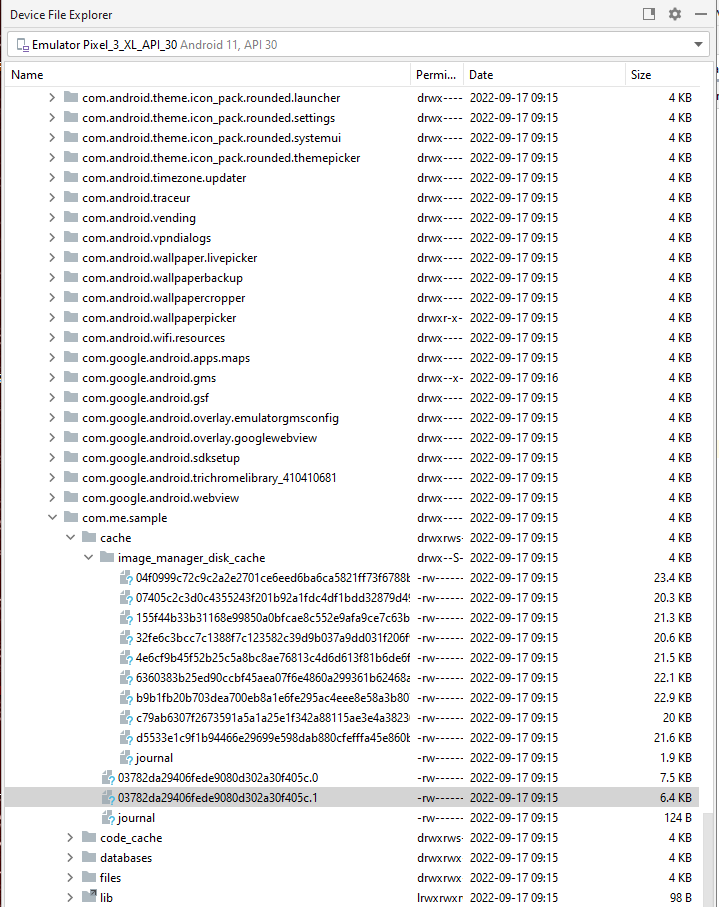
\includegraphics[width=.9\linewidth]{./pic/readme_20220917_093017.png}
\begin{itemize}
\item 能够把应用在前台(相当于应用的重新启动)或是后台被杀死后(系统有撮合接口供缓存)重建的情况优化,实现期望的逻辑;但是对图片的处理,好像仍然是从网上抓的图片,对图片的缓存与处理这块做得不够好
\item 第一次安装应用并运行的启动过程仍然很慢,图处的placeholder还没有设置好;
\item 最简单的对数据的处理没有处理好:当要求一个员工的数据必须五项都有的时候,可能有些数据是不全的;不过这个关系不大
\item 重大版块的逻辑都是实现了和连通好了的
\item 现在重新再次整合Room数据库,把手机内存产资源不足时销毁activity保存数据(应该需要的是持久性数据保存)的部分补充完整;
\item 一个极端情况下安卓手机内存不足时应用被系统杀死的数据保存与恢复需要数据库;这个地方想得还不是很透,可能把前面的问题解决了再解决这个极端用例
\item 这里模拟一下真机内存不足的时候杀进程,把它杀死,打个日志,分析一下,再进一步修改.试过上面一行Home后应用在后台杀死的方法,杀不掉;在前台倒是可以杀掉,抓个日志看一下
\end{itemize}
\begin{minted}[fontsize=\scriptsize,linenos=false]{ssh}
# 应用在前台强制关闭,强制停止指定的package包应用。
adb shell am force-stop com.me.sample 

# 应用通过home键已经停留在后台使用,杀死指定package包应用进程,该命令在安全模式下杀死进程,不影响用户体验。
# 参数选项:–user <USER_ID> | all | current: 指定user进程杀死,如果不指定默认为所有users。(关于USER_ID下面会介绍到)
# 可是这个方法杀不掉,应用还是最近应用列表里活着?【看着活着的是假的;它是真死了,留了个假象】
adb shell am kill com.me.sample 
adb shell ==> ps -A | grep com.me.sample # 前后对比就能够验证出,它是真死了

# 应用通过home键已经停留在后台使用,杀掉所有后台程序,需要先将目标程序按home进入后台,然后打开一个其他程序
# 可是这个方法杀不掉,应用还是最近应用列表里活着
adb shell am kill-all              
\end{minted}
\begin{itemize}
\item 应用被系统杀死后的重启,activity流程创建了两遍,是两个实例了吗?是,因为在onCreate()里两个实例reference的内存地址是不同的,所以是两个不同的实例。。。。。
\item 下面是应用被杀后,点击应用图标的重启过程,创建了两个实例
\end{itemize}
\begin{minted}[fontsize=\scriptsize,linenos=false]{text}
com.me.sample D/MainActivity: onCreate() 
com.me.sample I/ViewRootImpl@9fdb9bb[MainActivity]: setView = com.android.internal.policy.DecorView@ec3fbc TM=true
com.me.sample D/MainActivity: onStart() 
com.me.sample I/ViewRootImpl@9fdb9bb[MainActivity]: stopped(false) old=false
com.me.sample D/MainActivity: onResume() 
com.me.sample I/ViewRootImpl@e7eb0db[MainActivity]: setView = com.android.internal.policy.DecorView@798929f TM=true
com.me.sample I/ViewRootImpl@9fdb9bb[MainActivity]: Relayout returned: old=(0,142,1440,2872) new=(510,1297,930,1717) req=(420,420)0 dur=5 res=0x7 s={true -5476376617398110128} ch=true fn=-1
com.me.sample I/ViewRootImpl@9fdb9bb[MainActivity]: [DP] dp(1) 1 android.view.ViewRootImpl.reportNextDraw:11374 android.view.ViewRootImpl.performTraversals:4167 android.view.ViewRootImpl.doTraversal:2893 
com.me.sample I/BufferQueueProducer: [ViewRootImpl@9fdb9bb[MainActivity]#0(BLAST Consumer)0](id:297f00000000,api:1,p:10623,c:10623) queueBuffer: queued for the first time.
com.me.sample I/ViewRootImpl@e7eb0db[MainActivity]: Relayout returned: old=(0,0,1440,3040) new=(0,0,1440,3040) req=(1440,3040)0 dur=5 res=0x7 s={true -5476376617397988048} ch=true fn=-1
com.me.sample I/ViewRootImpl@e7eb0db[MainActivity]: [DP] dp(1) 1 android.view.ViewRootImpl.reportNextDraw:11374 android.view.ViewRootImpl.performTraversals:4167 android.view.ViewRootImpl.doTraversal:2893 
com.me.sample I/BufferQueueProducer: [ViewRootImpl@e7eb0db[MainActivity]#1(BLAST Consumer)1](id:297f00000001,api:1,p:10623,c:10623) queueBuffer: queued for the first time.
com.me.sample I/ViewRootImpl@e7eb0db[MainActivity]: [DP] pdf(0) 1 android.view.ViewRootImpl.lambda$addFrameCompleteCallbackIfNeeded$3$ViewRootImpl:4969 android.view.ViewRootImpl$$ExternalSyntheticLambda16.run:6 android.os.Handler.handleCallback:938 
com.me.sample I/ViewRootImpl@e7eb0db[MainActivity]: [DP] rdf()
com.me.sample D/ViewRootImpl@e7eb0db[MainActivity]: reportDrawFinished (fn: -1) 
com.me.sample I/ViewRootImpl@9fdb9bb[MainActivity]: [DP] pdf(0) 1 android.view.ViewRootImpl.lambda$addFrameCompleteCallbackIfNeeded$3$ViewRootImpl:4969 android.view.ViewRootImpl$$ExternalSyntheticLambda16.run:6 android.os.Handler.handleCallback:938 
com.me.sample I/ViewRootImpl@9fdb9bb[MainActivity]: [DP] rdf()
com.me.sample D/ViewRootImpl@9fdb9bb[MainActivity]: reportDrawFinished (fn: -1) 
com.me.sample I/ViewRootImpl@9fdb9bb[MainActivity]: dispatchDetachedFromWindow
com.me.sample I/ViewRootImpl@e7eb0db[MainActivity]: MSG_WINDOW_FOCUS_CHANGED 1 1
com.me.sample I/MainActivity: Started in onCreate(), running until onDestory(): 0
com.me.sample I/MainActivity: Started in onCreate(), running until onDestory(): 1
com.me.sample I/MainActivity: Started in onCreate(), running until onDestory(): 2

com.me.sample D/MainActivity: onCreate() 
com.me.sample I/ViewRootImpl@cfdc231[MainActivity]: setView = com.android.internal.policy.DecorView@11ea6c1 TM=true
com.me.sample D/MainActivity: onStart() 
com.me.sample I/ViewRootImpl@cfdc231[MainActivity]: stopped(false) old=false
com.me.sample D/MainActivity: onResume() 
com.me.sample I/ViewRootImpl@ccc5e51[MainActivity]: setView = com.android.internal.policy.DecorView@41dfb5 TM=true
com.me.sample I/ViewRootImpl@cfdc231[MainActivity]: Resizing android.view.ViewRootImpl@d4d842: frame=[510,1297][930,1717] reportDraw=true forceLayout=false backDropFrame=Rect(0, 0 - 420, 420)
com.me.sample I/ViewRootImpl@cfdc231[MainActivity]: Relayout returned: old=(0,142,1440,2872) new=(510,1297,930,1717) req=(420,420)0 dur=6 res=0x7 s={true -5476376617398049088} ch=true fn=-1
com.me.sample I/ViewRootImpl@cfdc231[MainActivity]: [DP] dp(1) 1 android.view.ViewRootImpl.reportNextDraw:11374 android.view.ViewRootImpl.performTraversals:4167 android.view.ViewRootImpl.doTraversal:2893 
com.me.sample I/BufferQueueProducer: [ViewRootImpl@cfdc231[MainActivity]#0(BLAST Consumer)0](id:2e8c00000000,api:1,p:11916,c:11916) queueBuffer: queued for the first time.
com.me.sample I/ViewRootImpl@ccc5e51[MainActivity]: Relayout returned: old=(0,0,1440,3040) new=(0,0,1440,3040) req=(1440,3040)0 dur=6 res=0x7 s={true -5476376617398005488} ch=true fn=-1
com.me.sample I/ViewRootImpl@ccc5e51[MainActivity]: [DP] dp(1) 1 android.view.ViewRootImpl.reportNextDraw:11374 android.view.ViewRootImpl.performTraversals:4167 android.view.ViewRootImpl.doTraversal:2893 
com.me.sample I/BufferQueueProducer: [ViewRootImpl@ccc5e51[MainActivity]#1(BLAST Consumer)1](id:2e8c00000001,api:1,p:11916,c:11916) queueBuffer: queued for the first time.
com.me.sample I/ViewRootImpl@ccc5e51[MainActivity]: [DP] pdf(0) 1 android.view.ViewRootImpl.lambda$addFrameCompleteCallbackIfNeeded$3$ViewRootImpl:4969 android.view.ViewRootImpl$$ExternalSyntheticLambda16.run:6 android.os.Handler.handleCallback:938 
com.me.sample I/ViewRootImpl@ccc5e51[MainActivity]: [DP] rdf()
com.me.sample D/ViewRootImpl@ccc5e51[MainActivity]: reportDrawFinished (fn: -1) 
com.me.sample I/ViewRootImpl@cfdc231[MainActivity]: [DP] pdf(0) 1 android.view.ViewRootImpl.lambda$addFrameCompleteCallbackIfNeeded$3$ViewRootImpl:4969 android.view.ViewRootImpl$$ExternalSyntheticLambda16.run:6 android.os.Handler.handleCallback:938 
com.me.sample I/ViewRootImpl@cfdc231[MainActivity]: [DP] rdf()
com.me.sample D/ViewRootImpl@cfdc231[MainActivity]: reportDrawFinished (fn: -1) 
com.me.sample I/ViewRootImpl@cfdc231[MainActivity]: handleResized, msg = 5 frames=ClientWindowFrames{frame=[510,1297][930,1717] display=[0,142][1440,2872] backdrop=[0,0][420,420]} forceNextWindowRelayout=false displayId=0 frameChanged=false backdropFrameChanged=true configChanged=false displayChanged=false mNextDrawUseBlastSync=false mergedConfiguration={mGlobalConfig={1.1 311mcc480mnc [en_US] ldltr sw411dp w411dp h780dp 560dpi nrml long hdr widecg port finger -keyb/v/h -nav/h winConfig={ mBounds=Rect(0, 0 - 1440, 3040) mAppBounds=Rect(0, 142 - 1440, 2872) mMaxBounds=Rect(0, 0 - 1440, 3040) mWindowingMode=fullscreen mDisplayWindowingMode=fullscreen mActivityType=undefined mAlwaysOnTop=undefined mRotation=ROTATION_0 mPopOver=off mFreeformTaskPinningState=unpinned} s.26854 fontWeightAdjustment=0 ff=0 bf=0 bts=0 desktop/d dm/n dc/d ?dcui ?dcaf enb/d themeSeq=0} mOverrideConfig={1.1 311mcc480mnc [en_US] ldltr sw411dp w411dp h780dp 560dpi nrml long hdr widecg port finger -keyb/v/h -nav/h winConfig={ mBounds=Rect(0, 0 - 1440, 3040) mAppBounds=Rect(0, 142 - 1440, 2872) mMaxBounds=Rect(0, 0 - 1440, 3040) mWindowingMode=fullscreen mDisplayWindowingMode=fullscreen mActivityType=standard mAlwaysOnTop=undefined mRotation=ROTATION_0 mPopOver=off mFreeformTaskPinningState=unpinned} s.1 fontWeightAdjustment=0 ff=0 bf=0 bts=0 desktop/d dm/n dc/d ?dcui ?dcaf enb/d themeSeq=0}}
com.me.sample I/ViewRootImpl@cfdc231[MainActivity]: [DP] dp(1) 1 android.view.ViewRootImpl.reportNextDraw:11374 android.view.ViewRootImpl.handleResized:2204 android.view.ViewRootImpl.access$1200:294
\end{minted}
\begin{itemize}
\item 从最近应用列表点击图标,重启过程会是怎样的呢?
\end{itemize}
\begin{minted}[fontsize=\scriptsize,linenos=false]{text}
com.me.sample D/MainActivity: onCreate() 
com.me.sample I/ViewRootImpl@1413ed8[MainActivity]: setView = com.android.internal.policy.DecorView@11529a TM=true
com.me.sample D/MainActivity: onStart() 
com.me.sample D/MainActivity: onRestoreInstanceState() 
com.me.sample I/ViewRootImpl@1413ed8[MainActivity]: stopped(false) old=false
com.me.sample D/MainActivity: onResume() 
com.me.sample I/ViewRootImpl@a363778[MainActivity]: setView = com.android.internal.policy.DecorView@e9d0fec TM=true
com.me.sample I/ViewRootImpl@1413ed8[MainActivity]: Relayout returned: old=(0,142,1440,2872) new=(510,1297,930,1717) req=(420,420)0 dur=5 res=0x7 s={true -5476376617398040368} ch=true fn=-1
com.me.sample I/ViewRootImpl@1413ed8[MainActivity]: [DP] dp(1) 1 android.view.ViewRootImpl.reportNextDraw:11374 android.view.ViewRootImpl.performTraversals:4167 android.view.ViewRootImpl.doTraversal:2893 
com.me.sample I/BufferQueueProducer: [ViewRootImpl@1413ed8[MainActivity]#0(BLAST Consumer)0](id:610c00000000,api:1,p:24844,c:24844) queueBuffer: queued for the first time.
com.me.sample I/ViewRootImpl@a363778[MainActivity]: Relayout returned: old=(0,0,1440,3040) new=(0,0,1440,3040) req=(1440,3040)0 dur=4 res=0x7 s={true -5476376617398005488} ch=true fn=-1
com.me.sample I/ViewRootImpl@a363778[MainActivity]: [DP] dp(1) 1 android.view.ViewRootImpl.reportNextDraw:11374 android.view.ViewRootImpl.performTraversals:4167 android.view.ViewRootImpl.doTraversal:2893 
com.me.sample I/BufferQueueProducer: [ViewRootImpl@a363778[MainActivity]#1(BLAST Consumer)1](id:610c00000001,api:1,p:24844,c:24844) queueBuffer: queued for the first time.
com.me.sample I/ViewRootImpl@a363778[MainActivity]: [DP] pdf(0) 1 android.view.ViewRootImpl.lambda$addFrameCompleteCallbackIfNeeded$3$ViewRootImpl:4969 android.view.ViewRootImpl$$ExternalSyntheticLambda16.run:6 android.os.Handler.handleCallback:938 
com.me.sample I/ViewRootImpl@a363778[MainActivity]: [DP] rdf()
com.me.sample D/ViewRootImpl@a363778[MainActivity]: reportDrawFinished (fn: -1) 
com.me.sample I/ViewRootImpl@1413ed8[MainActivity]: [DP] pdf(0) 1 android.view.ViewRootImpl.lambda$addFrameCompleteCallbackIfNeeded$3$ViewRootImpl:4969 android.view.ViewRootImpl$$ExternalSyntheticLambda16.run:6 android.os.Handler.handleCallback:938 
com.me.sample I/ViewRootImpl@1413ed8[MainActivity]: [DP] rdf()
com.me.sample D/ViewRootImpl@1413ed8[MainActivity]: reportDrawFinished (fn: -1) 
com.me.sample I/ViewRootImpl@1413ed8[MainActivity]: dispatchDetachedFromWindow
com.me.sample I/ViewRootImpl@a363778[MainActivity]: MSG_WINDOW_FOCUS_CHANGED 1 1
\end{minted}
\begin{itemize}
\item 当把应用杀死:再重建,去检查安卓系统帮保存或是恢复了什么,却发现大概是因为使用了第三方库根不上配置的原因,被杀后的重建视图会成为一片空白。所以这里就一定要修改重建逻辑了
\end{itemize}

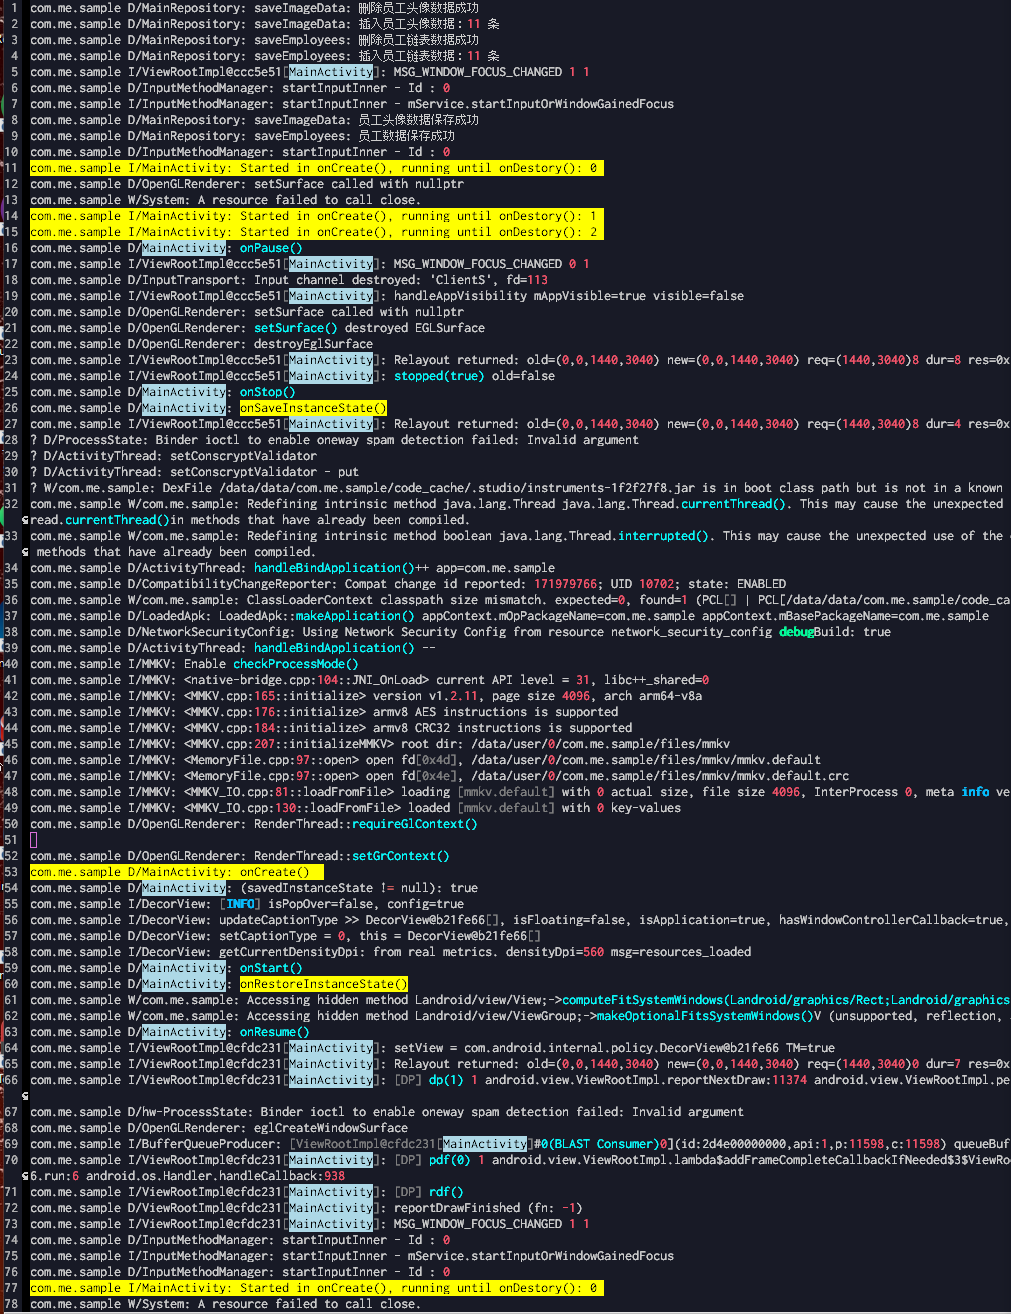
\includegraphics[width=.9\linewidth]{./pic/readme_20220915_225835.png}
\begin{minted}[fontsize=\scriptsize,linenos=false]{text}
com.me.sample D/MainRepository: saveImageData: 删除员工头像数据成功
com.me.sample D/MainRepository: saveImageData: 插入员工头像数据:11条
com.me.sample D/MainRepository: saveEmployees: 删除员工链表数据成功
com.me.sample D/MainRepository: saveEmployees: 插入员工链表数据:11条
com.me.sample I/ViewRootImpl@ccc5e51[MainActivity]: MSG_WINDOW_FOCUS_CHANGED 1 1
com.me.sample D/InputMethodManager: startInputInner - Id : 0
com.me.sample I/InputMethodManager: startInputInner - mService.startInputOrWindowGainedFocus
com.me.sample D/MainRepository: saveImageData: 员工头像数据保存成功
com.me.sample D/MainRepository: saveEmployees: 员工数据保存成功
com.me.sample D/InputMethodManager: startInputInner - Id : 0
com.me.sample I/MainActivity: Started in onCreate(), running until onDestory(): 0
com.me.sample D/OpenGLRenderer: setSurface called with nullptr
com.me.sample W/System: A resource failed to call close. 
com.me.sample I/MainActivity: Started in onCreate(), running until onDestory(): 1
com.me.sample I/MainActivity: Started in onCreate(), running until onDestory(): 2
com.me.sample D/MainActivity: onPause() 
com.me.sample I/ViewRootImpl@ccc5e51[MainActivity]: MSG_WINDOW_FOCUS_CHANGED 0 1
com.me.sample D/InputTransport: Input channel destroyed: 'ClientS', fd=113
com.me.sample I/ViewRootImpl@ccc5e51[MainActivity]: handleAppVisibility mAppVisible=true visible=false
com.me.sample D/OpenGLRenderer: setSurface called with nullptr
com.me.sample D/OpenGLRenderer: setSurface() destroyed EGLSurface
com.me.sample D/OpenGLRenderer: destroyEglSurface
com.me.sample I/ViewRootImpl@ccc5e51[MainActivity]: Relayout returned: old=(0,0,1440,3040) new=(0,0,1440,3040) req=(1440,3040)8 dur=8 res=0x5 s={false 0} ch=true fn=7
com.me.sample I/ViewRootImpl@ccc5e51[MainActivity]: stopped(true) old=false
com.me.sample D/MainActivity: onStop() 
com.me.sample D/MainActivity: onSaveInstanceState()
com.me.sample I/ViewRootImpl@ccc5e51[MainActivity]: Relayout returned: old=(0,0,1440,3040) new=(0,0,1440,3040) req=(1440,3040)8 dur=4 res=0x5 s={false 0} ch=false fn=-1
? I/com.me.sample: Late-enabling -Xcheck:jni
? E/USNET: USNET: appName: com.me.sample
? D/ProcessState: Binder ioctl to enable oneway spam detection failed: Invalid argument
? D/ActivityThread: setConscryptValidator
? D/ActivityThread: setConscryptValidator - put
? W/com.me.sample: DexFile /data/data/com.me.sample/code_cache/.studio/instruments-1f2f27f8.jar is in boot class path but is not in a known location
com.me.sample W/com.me.sample: Redefining intrinsic method java.lang.Thread java.lang.Thread.currentThread(). This may cause the unexpected use of the original definition of java.lang.Thread java.lang.Thread.currentThread()in methods that have already been compiled.
com.me.sample W/com.me.sample: Redefining intrinsic method boolean java.lang.Thread.interrupted(). This may cause the unexpected use of the original definition of boolean java.lang.Thread.interrupted()in methods that have already been compiled.
com.me.sample D/ActivityThread: handleBindApplication()++ app=com.me.sample
com.me.sample D/CompatibilityChangeReporter: Compat change id reported: 171979766; UID 10702; state: ENABLED
com.me.sample W/com.me.sample: ClassLoaderContext classpath size mismatch. expected=0, found=1 (PCL[] | PCL[/data/data/com.me.sample/code_cache/.overlay/base.apk/classes14.dex*1294054685])
com.me.sample D/LoadedApk: LoadedApk::makeApplication() appContext.mOpPackageName=com.me.sample appContext.mBasePackageName=com.me.sample
com.me.sample D/NetworkSecurityConfig: Using Network Security Config from resource network_security_config debugBuild: true
com.me.sample D/ActivityThread: handleBindApplication() --
com.me.sample I/MMKV: Enable checkProcessMode()
com.me.sample I/MMKV: <native-bridge.cpp:104::JNI_OnLoad> current API level = 31, libc++_shared=0
com.me.sample I/MMKV: <MMKV.cpp:165::initialize> version v1.2.11, page size 4096, arch arm64-v8a
com.me.sample I/MMKV: <MMKV.cpp:176::initialize> armv8 AES instructions is supported
com.me.sample I/MMKV: <MMKV.cpp:184::initialize> armv8 CRC32 instructions is supported
com.me.sample I/MMKV: <MMKV.cpp:207::initializeMMKV> root dir: /data/user/0/com.me.sample/files/mmkv
com.me.sample I/MMKV: <MemoryFile.cpp:97::open> open fd[0x4d], /data/user/0/com.me.sample/files/mmkv/mmkv.default
com.me.sample I/MMKV: <MemoryFile.cpp:97::open> open fd[0x4e], /data/user/0/com.me.sample/files/mmkv/mmkv.default.crc
com.me.sample I/MMKV: <MMKV_IO.cpp:81::loadFromFile> loading [mmkv.default] with 0 actual size, file size 4096, InterProcess 0, meta info version:1
com.me.sample I/MMKV: <MMKV_IO.cpp:130::loadFromFile> loaded [mmkv.default] with 0 key-values
com.me.sample D/OpenGLRenderer: RenderThread::requireGlContext()

com.me.sample D/OpenGLRenderer: RenderThread::setGrContext()
com.me.sample D/MainActivity: onCreate() 
com.me.sample D/MainActivity: (savedInstanceState != null): true
com.me.sample I/DecorView: [INFO] isPopOver=false, config=true
com.me.sample I/DecorView: updateCaptionType >> DecorView@b21fe66[], isFloating=false, isApplication=true, hasWindowControllerCallback=true, hasWindowDecorCaption=false
com.me.sample D/DecorView: setCaptionType = 0, this = DecorView@b21fe66[]
com.me.sample I/DecorView: getCurrentDensityDpi: from real metrics. densityDpi=560 msg=resources_loaded
com.me.sample D/MainActivity: onStart() 
com.me.sample D/MainActivity: onRestoreInstanceState() 
com.me.sample W/com.me.sample: Accessing hidden method Landroid/view/View;->computeFitSystemWindows(Landroid/graphics/Rect;Landroid/graphics/Rect;)Z (unsupported, reflection, allowed)
com.me.sample W/com.me.sample: Accessing hidden method Landroid/view/ViewGroup;->makeOptionalFitsSystemWindows()V (unsupported, reflection, allowed)
com.me.sample D/MainActivity: onResume() 
com.me.sample I/ViewRootImpl@cfdc231[MainActivity]: setView = com.android.internal.policy.DecorView@b21fe66 TM=true
com.me.sample I/ViewRootImpl@cfdc231[MainActivity]: Relayout returned: old=(0,0,1440,3040) new=(0,0,1440,3040) req=(1440,3040)0 dur=7 res=0x7 s={true -5476376617398057808} ch=true fn=-1
com.me.sample I/ViewRootImpl@cfdc231[MainActivity]: [DP] dp(1) 1 android.view.ViewRootImpl.reportNextDraw:11374 android.view.ViewRootImpl.performTraversals:4167 android.view.ViewRootImpl.doTraversal:2893 
com.me.sample D/hw-ProcessState: Binder ioctl to enable oneway spam detection failed: Invalid argument
com.me.sample D/OpenGLRenderer: eglCreateWindowSurface
com.me.sample I/BufferQueueProducer: [ViewRootImpl@cfdc231[MainActivity]#0(BLAST Consumer)0](id:2d4e00000000,api:1,p:11598,c:11598) queueBuffer: queued for the first time.
com.me.sample I/ViewRootImpl@cfdc231[MainActivity]: [DP] pdf(0) 1 android.view.ViewRootImpl.lambda$addFrameCompleteCallbackIfNeeded$3$ViewRootImpl:4969 android.view.ViewRootImpl$$ExternalSyntheticLambda16.run:6 android.os.Handler.handleCallback:938 
com.me.sample I/ViewRootImpl@cfdc231[MainActivity]: [DP] rdf()
com.me.sample D/ViewRootImpl@cfdc231[MainActivity]: reportDrawFinished (fn: -1) 
com.me.sample I/ViewRootImpl@cfdc231[MainActivity]: MSG_WINDOW_FOCUS_CHANGED 1 1
com.me.sample D/InputMethodManager: startInputInner - Id : 0
com.me.sample I/InputMethodManager: startInputInner - mService.startInputOrWindowGainedFocus
com.me.sample D/InputMethodManager: startInputInner - Id : 0
com.me.sample I/MainActivity: Started in onCreate(), running until onDestory(): 0
com.me.sample W/System: A resource failed to call close.
\end{minted}
\begin{itemize}
\item 现在就真正到了 \textbf{要自己调控应用被系统杀死的重启过程了} ,hihi
\item 这里会分为当活动(activitty被系统杀死的时候,应用是否被系统杀死的情况)来把这单个活动的恢复,和或整个应用被杀死后的重启过程搞清楚,如何优化启动过程,以及规避不必要的网络请求等。今天是晚上回家后再接着把这个部分弄懂弄透写完
\item 需要找一找大电脑上还有没有先前写的日志文件syslog-mode的关键词parser传上去,笔记上会需要用到;同步先前所修改过的syslog-mode相关的所有emacs bug到window系统上,明天要用
\item 总结一下:onSaveInstanceState 只能保存少量数据,ViewModel 只能保存数据到内存。所以对于更大的数据状态保存我们应该放在磁盘文件中或者使用数据库处理。
\item 比如这样一个场景,我们的应用是一个 im 的即时通讯 app。在聊天列表页面,每次更新了列表中的联系人窗口数据都会使用数据库进行存储。那么就有一下三种场景了:
\begin{itemize}
\item Activity 初次创建,或是用户点击了网络请求的按钮之后,网络请求,刷新UI,并(每有刷新都第二时间,第一时间UI)同步数据到数据库
\item Activity 配置发生更改导致 Activity 被重建(不需要网络刷新,直接使用ViewModel里内存里的现存数据)
\item Activity 所在进程被系统回收,再次进入被重建
\end{itemize}
\item 针对 1:刚进入 Activity 的时候我们需要请求后台查看有没有增量的联系人,如果有拉取数据存储在本地数据库。还是使用轻量的sharedPreference来保存是否有数据库的数据。分两种情况:第一次创建以及用户要求刷新时,刷新并保存网络数据;其它任何时候都只从数据库读取现胡有数据
\item 针对 2:的情况,Activity 被重建的时候,因为 ViewModel 没有被销毁,我们可以直接从 ViewModel 中恢复数据,不需要请求网络(当然了你为了保持数据的实时性去请求也无可厚非)
\item 针对 3:的情况,我们可以在 onSaveInstanceState 中保存联系人的 id,Activity 被重建的时候拿到这个 id 去数据库中查找数据,这种情况也不需要请求网络。(当然了你为了保持数据的实时性去请求也无可厚非)
\item 现在存在问题:
\begin{itemize}
\item \textbf{测试模块还没有写(有一个系统自带的测试用例,不想写这个模块了)}
\item 网络请求可能存在内存泄露(比如,使用RxJava发布一个订阅后,当Activity被finish,此时订阅逻辑还未完成,如果没有及时取消订阅,就会导致Activity无法被回收,从而引发内存泄漏);写往数据库的部分因为使用了CompositeDisposable可能没有这个问题;
\item 现在应用恢复正常运行,并且移除了Hilt的自动注入,不再存在Hilt与RxLifeCycle不合作的问题,先(今天晚上)把这个内存泄露问题给解决了;(参考消息: \url{https://www.jianshu.com/p/8311410de676})
\begin{itemize}
\item 这个问题太好解决了,虽然原理都还木有弄懂。。。。。明天早上再看一下
\item 去了解一下一个更为优秀的库: \textbf{用AutoDisposable来代替RxLifeCycle来解决网络请求过程中可能会出现的内存泄露问题; 明天早上再看一下这个问题的原理} \url{https://blog.csdn.net/fitaotao/article/details/117519733}
\end{itemize}
\item 目前网上对RxJava的内存泄漏有几种方案:(现实现了RxLifeCycle里的防止,可以再试一下AutoDisposable第三方库,暂时先这样)
\begin{itemize}
\item 通过封装,手动为RxJava的每一次订阅进行控制,在指定的时机进行取消订阅;
\item 使用 Daniel Lew 的 RxLifecycle ,通过监听Activity、Fragment的生命周期,来自动断开subscription以防止内存泄漏。
\end{itemize}
\end{itemize}
\item 现在终于改掉了自己网址写错的小bug了,可以再往前迈进一步,深入深解拦截器与OkHttp底层的原理了。。。
\item 顺着这个例子\url{https://github.com/xitu/gold-miner/blob/master/TODO/getting-started-with-retrofit.md} 把进阶的部分看完,弄懂
\item 终于找到了先前 \textbf{今年二三月份参考过的一个很好的案例日志序列} : MVVM \url{https://blog.csdn.net/qq_38436214/category_11482619.html?spm=1001.2014.3001.5482}
\begin{itemize}
\item 下午忘记带一根测试用的线了,就暂时理一下思路,晚上回家后再在大电脑上测试
\end{itemize}
\item 这是一个 \textbf{看似要求极其简单,实则考验的知识点和深度有着相当的跨度的小项目。}
\item 它们一定挑都要挑我出差到WSU的一个星期里来考验我,因为他们就是想要去打败一个人。呵呵,真正想要打败一个人,谈何容易,就凭这???
\item \textbf{Retrofit + RxJava}: 好像是更合适的,可以用注解,并且用得更为广泛
\begin{itemize}
\item 搜索关键字:Retrofit + OkHttp +RxJava 网络库构建
\item \textbf{OkHttp}: 网络请求处理,主要是在应用启动的时候,什么时机开始发布和调用网络请求。所以这个可以不用了,大家都喜欢新的更好用的库
\end{itemize}
\item \textbf{网络数据解析} :我这里得到了网络数据,可是好像我并没有解析数据出来,这整个过程我可能还少了这比较关键的一个步骤
\begin{itemize}
\item 当对这类框架和OOP设计有了更好的了解,就可以自定义解析类来在获得数据前自动解析为自己想要的类型
\begin{itemize}
\item 注意这里提供的API其实并没有code msg之类的信息,而是直接的结果;再想一下:为什么OkHttp的拦截器能够得到code 200呢?这里Response返回基本信息还有点儿糊涂
\item 可以参考这个例子: \url{https://developer.aliyun.com/article/609862}
\end{itemize}
\end{itemize}
\item \textbf{RxJava基本原理} :RxJava is a Java VM implementation of Reactive Extensions: a library for composing asynchronous and event-based programs by using observable sequences.(一个通过使用可观察序列来组成异步的、基于事件的程序的库。)
\begin{itemize}
\item 从介绍中我们可以提取出一个关键词:异步,但安卓中已经有很多解决异步操作的方法了,比如Handler和AsyncTask等, \textbf{为什么还选择RxJava呢,其实目的就是为了让代码更简洁,而且它的简洁是与众不同的,因为RxJava的使用方式是基于事件流的链式调用,这就保证了随着程序复杂性的提高,RxJava依然能保持代码的简洁和优雅} 。
\end{itemize}
\item \textbf{图片本地缓存}: 第三方库找一个,还是用AndroidX的Room
\begin{itemize}
\item 上面可能想错了,就是使用的第三方图片库Glide本身已经具备了缓存图片到本地的功能,所有我大可不必再多此一举,再来一个AndroidX Jetpack的Room数据库
\item 现将所有的room数据库相送的源码全部删除, \textbf{现只负责将RecyclerView的所有相送逻辑连通就可以了}
\end{itemize}
\item 小问题:根据返回来数据的url链接来加载员工头像图片,可能并不需要我来实现什么网络请求的串接执行,更多应该是 \textbf{Recyclerview的双向数据绑定就可以了}
\item 头像图片加载:现有两套思路,一套Mitch的MVVM但是非数据绑定的版本,一套双向数据绑定的自动化绑定的版本。
\begin{itemize}
\item 按照项目的要求与缓存机制的要求,我觉得用Mitch的版本更为简洁,主要由第三方库Glide帮助缓存处理。自己需要必理的逻辑比较少,更简洁方便好用。
\item 那么下面的这些关于缓存的问题都可以暂时不思考了,先运行起一个可以执行运行不出错的应用再说再优化。
\item 我 \textbf{现在数据库的问题} 是:我 \textbf{缓存保存了员工数据进数据库} ,但是这里说得很清楚了, \textbf{不用保存员工数据,只保存每个员工id所对应的图片就可以了}
\item 说到网络缓存,肯定都不陌生,多多少少使用过不同的缓存方案。使用网络缓存有什么作用:
\begin{itemize}
\item 减少服务器请求次数
\item 减少用户等待时间
\item 增加应用流畅度
\item 节省用户流量(虽然现在流量也不怎么值钱了)
\end{itemize}
\end{itemize}
\item 应用的 \textbf{启动优化} :重中之重,需要借助这个小应用弄懂弄清楚, \textbf{不知道如何拆解网络请求的步骤,什么时候加载,初始化之类的?} 以达到较好的启动优化
\item \textbf{MVVM设计} :只有一个页面,相对就简单方便多了。工作中的案例是使用MVVM但自己编辑逻辑处理信号下发,与数据驱动的UI更新,没有实现双向数据绑定的;可是这里感觉 \textbf{双向数据绑定} 更简单,会有哪些可能的问题呢?这里基本可以当作不需要双向,因为一个UI按钮要求刷新是唯一的UI需求;更多的只是需要时候的数据往UI加载更新;所以 \textbf{可以简单使用观察者模式,UI观察数据的变化} 就可以了
\item \textbf{图片的加载与处理} :用样可以使用么第三方库 \textbf{glide}
\item \textbf{图片的加载与处理} :用样可以使用么第三方库 \textbf{CircularImageView}
\item \textbf{AndroidX RecyclerView} 的使用:选择相对更为高效和方便管理的库和数据结构来使用
\item \textbf{Constraint Layout vs Coordinate Layout}: 暂时先用任何简单的layout先能运行起一个大致的框架来,再进一步优化
\item 我丢掉了的文件呀,我写过的项目呀,不是在进Lucid之前写得好好的一个项目,现在源码全丢了。。。。。该死的GitHub\ldots{}..
\end{itemize}
\section{OkHttp网络请求的缓存}
\label{sec-3}
\begin{itemize}
\item \textbf{OkHttpClient/Retrofit里在网络请求的时候(根据不同的url链接,或是不是请求接口?基于拦截器来做缓存)来动态使用不同的缓存策略(适用于自己只缓存图片,而不缓存员工链表)} ,这个思路应该用在这个项目的设计与实现里。原理参考这个思路: 
\begin{itemize}
\item \url{https://blog.csdn.net/c10WTiybQ1Ye3/article/details/125687902?spm=1001.2101.3001.6661.1&utm_medium=distribute.pc_relevant_t0.none-task-blog-2\%7Edefault\%7ECTRLIST\%7ERate-1-125687902-blog-51550400.pc_relevant_multi_platform_whitelistv3&depth_1-utm_source=distribute.pc_relevant_t0.none-task-blog-2\%7Edefault\%7ECTRLIST\%7ERate-1-125687902-blog-51550400.pc_relevant_multi_platform_whitelistv3&utm_relevant_index=1}
\end{itemize}
\item 笔记本电脑上的kotlin-mode还没有配置好,改天配置好后再把这个部分的代码好好整理一下。早上时间紧张,暂时没时间来处理这个了
\end{itemize}
\begin{minted}[fontsize=\scriptsize,linenos=false]{kotlin}
private fun buildCacheKey(request: Request): String {
    val requestBody = request.body ?: return request.url.toString()
    val buffer = Buffer()
    requestBody.writeTo(buffer)

    val contentType = requestBody.contentType()
    val charset = contentType?.charset(Charsets.UTF_8) ?: Charsets.UTF_8

    if (isProbablyUtf8(buffer)) {
        val questParam = buffer.readString(charset)
        buffer.close()
        if (questParam.isBlank()) return request.url.toString()
        val builder = request.url.newBuilder()
        kotlin.runCatching {
            builder.addQueryParameter("${request.method.lowercase()}param", questParam)
            return builder.build().toString()
        }.onFailure {
            return ""
        }
    }
    return request.url.toString()
}

// 拦截器
// 我们在拦截器里做缓存,每次请求可能会是不同的策略,所以首先要拿到的就是缓存模式,
// 拿到缓存模式之后再根据不同的模式去读取或者写入操作,核心代码也就下边这几行:
override fun intercept(chain: Interceptor.Chain): Response {
    val initialRequest = chain.request()
    val strategy = CacheUtil.getCacheStrategy(initialRequest)
    val newRequest = initialRequest.rmCacheHeader()

    if (strategy == null) return chain.proceed(newRequest)// 策略为空,直接返回网络结果

    // ONLY_NETWORK 直接请求网络
    if (strategy.cacheMode == CacheMode.ONLY_NETWORK) return chain.proceed(newRequest)

    // ONLY_CACHE 只读取缓存
    if (strategy.cacheMode == CacheMode.ONLY_CACHE) {
        // 只读缓存模式,缓存为空,返回错误响应
        return (if (CacheManager.useExpiredData) mCache.getCache(strategy.cacheKey, newRequest)
                else redCache(strategy, newRequest)) ?: Response.Builder()
            .request(chain.request())
            .protocol(Protocol.HTTP_1_1)
            .code(HttpURLConnection.HTTP_GATEWAY_TIMEOUT)
            .message("no cached data")
            .body(EMPTY_RESPONSE)
            .sentRequestAtMillis(-1L)
            .receivedResponseAtMillis(System.currentTimeMillis())
            .build()
    }

    //先取缓存再取网络
    if (strategy.cacheMode == CacheMode.READ_CACHE_NETWORK_PUT) {
        val cacheResponse = redCache(strategy, newRequest)
        if (cacheResponse != null) return cacheResponse
    }

    try {
        // 开始请求网络
        val response = chain.proceed(newRequest)
        // 成功后写入缓存
        if (response.isSuccessful) {
            return cacheWritingResponse(mCache.putCache(strategy.cacheKey, response), response)
        }
        if (strategy.cacheMode == CacheMode.NETWORK_PUT_READ_CACHE) {
            return redCache(strategy, newRequest) ?: response
        }
        return response
    } catch (e: Throwable) {
        //请求失败尝试读取缓存,缓存没有或者失效,抛异常
        if (strategy.cacheMode == CacheMode.NETWORK_PUT_READ_CACHE) {
            return redCache(strategy, newRequest) ?: throw e
        }
        throw e
    }
}

// 设置缓存
// 这里不得不佩服 Retrofit 在解耦方面做的是真的强啊。我何时能有那样的思路跟想法呢。眼里只有崇拜~~~
// 言归正传 Retrofit 的请求头是在 Service里边添加的,所以添加缓存策略,直接写在Service里。
// Retrofit 两种添加请求头的方式@Headers 是方法注解,@Header 是参数注解。
// 再结合Kotlin 语法可以指定默认参数,如有不同缓存模式就可以在请求的时候,去动态使用不同缓存模式。
/**
 * 使用 Header 参数注解
 */
@FormUrlEncoded
@POST("user/login")
suspend fun login(
    @Field("username") username: String,
    @Field("password") password: String,
    @Header(CacheStrategy.CACHE_MODE) cacheMode: String = CacheMode.READ_CACHE_NETWORK_PUT,
    @Header(CacheStrategy.CACHE_TIME) cacheTime: String = "10"// 过期时间,10秒 不过期
): BaseResponse<Any>

/**
 * 使用 Headers 方法注解
 */
@Headers(
    "${CacheStrategy.CACHE_TIME}:-1", // 过期时间,-1 不过期
    "${CacheStrategy.CACHE_MODE}:${CacheMode.READ_CACHE_NETWORK_PUT}"
)
@GET("article/list/{page}/json")
suspend fun getPage(@Path("page") page: Any): BaseResponse<Page<ArticleBean>>

// 缓存的读写
// 读写操作还是用的OkHttp 的 DiskLruCache类。
// Okhttp 4.0.0 版本以后 就用 Kotlin 重构了。DiskLruCache 的构造函数被 internal 修饰了。
// 重构后的前几个版本还提供了 静态方法来创建。后边版本直接静态方法都移除了,这是要搞事情啊,不准备给我们用的样子。
// 不过如果用Java写的话就可以直接创建,Java会忽视 internal 关键字直接过编译期。但是 Kotlin 就不行了,会报错。
// 又不想用Java写。还是直接用反射创建吧,没有反射干不了的事情。
internal fun getDiskLruCache(
    fileSystem: FileSystem?,
    directory: File?,
    appVersion: Int,
    valueCount: Int,
    maxSize: Long
): DiskLruCache {
    val cls = DiskLruCache::class.java
    return try {
        val runnerClass = Class.forName("okhttp3.internal.concurrent.TaskRunner")
        val constructor = cls.getConstructor(
            FileSystem::class.java,
            File::class.java,
            Int::class.java,
            Int::class.java,
            Long::class.java,
            runnerClass
        )
        constructor.newInstance(
            fileSystem,
            directory,
            appVersion,
            valueCount,
            maxSize,
            TaskRunner.INSTANCE
        )
    } catch (e: Exception) {
        try {
            val constructor = cls.getConstructor(
                FileSystem::class.java,
                File::class.java,
                Int::class.java,
                Int::class.java,
                Long::class.java,
                Executor::class.java
            )
            val executor = ThreadPoolExecutor(
                0, 1, 60L, TimeUnit.SECONDS,
                LinkedBlockingQueue(), threadFactory("OkHttp DiskLruCache", true)
            )
            constructor.newInstance(
                fileSystem,
                directory,
                appVersion,
                valueCount,
                maxSize,
                executor
            )
        } catch (e: Exception) {
            throw IllegalArgumentException("Please use okhttp 4.0.0 or later")
        }
    }
}
// 刚好4.0.0 之后的几个版本,构造函数要提供一个线程池,4.3.0 后的版本成了 TaskRunner 了。可以都兼容一下。
// 具体的读写IO操作在CacheManager.kt 这个类中,这个是根据Okhttp 的 Cache 修改而来的。
// 全局参数
// 增加了全局 设置缓存模式、缓存时间。优先级还是 Service 中声明出来的高。
CacheManager.setCacheModel(CacheMode.READ_CACHE_NETWORK_PUT)// 设置全局缓存模式
    .setCacheTime(15 * 1000) // 设置全局 过期时间 (毫秒)
    .useExpiredData(true)// 缓存过期时是否继续使用,仅对 ONLY_CACHE 生效
// 具体使用方式:详见Demo NetCache: https://github.com/AleynP/net-cache
\end{minted}
\begin{itemize}
\item 现在的难点:不知道怎么定义图片数据库,同时以OkHTTP respnose回来的连接起来 (可以参考下面的一个例子,虽然MVVM的分工可能还不是很明确,但至少是一个可以运行的版本)
\end{itemize}

\section{封装:OkHttp + EventBus}
\label{sec-4}
\begin{itemize}
\item EventBut是自己知识点面上的欠缺。借助这个极小的包装,打开一个通向真正理解这个OkHttp底层EventBus的道路。。。。
\item event有5个类: \textbf{BaseEvent + HttpEvent + HttpSuccessEvent + HttpErrorEvent + AppEvent}
\item \textbf{RequestTag}:请求tag
\item \textbf{MainReqeust}:封装了OkHttp的回调,onResponse(\ldots{}) onFailure(\ldots{})中用EventBus发送数据
\item \textbf{UserRequest} :请求网络数据的方法全部在里面,把OkHttp的前3步写在这里面,第4布封装在了MainRequest中
\item \textbf{BaseActivity}:订阅事件总线,接收EventBus发送(post)的数据
\end{itemize}
\subsection{BaseEvent.java}
\label{sec-4-1}
\begin{minted}[fontsize=\scriptsize,linenos=false]{csharp}
public class BaseEvent {
    private int id;
    private String message;
    public int getId() {
        return id;
    }
    public void setId(int id) {
        this.id = id;
    }
    public String getMessage() {
        return message;
    }
    public void setMessage(String message) {
        this.message = message;
    }
}
\end{minted}
\subsection{HttpEvent}
\label{sec-4-2}
\begin{minted}[fontsize=\scriptsize,linenos=false]{csharp}
public class HttpEvent extends BaseEvent {
    @NonNull
        private RequestTag requestTag;
    public RequestTag getRequestTag() {
        return requestTag;
    }
    public void setRequestTag(@NonNull RequestTag requestTag) {
        this.requestTag = requestTag;
    }
}
\end{minted}
\subsection{HttpSuccessEvent}
\label{sec-4-3}
\begin{minted}[fontsize=\scriptsize,linenos=false]{csharp}
public class HttpSuccessEvent extends HttpEvent {
    
    private String json;
    public String getJson() {
        return json;
    }
    public void setJson(String json) {
        this.json = json;
    }
}
\end{minted}
\subsection{HttpErrorEvent}
\label{sec-4-4}
\begin{minted}[fontsize=\scriptsize,linenos=false]{csharp}
public class HttpErrorEvent extends HttpEvent {
    private int errorCode;
    private String errorMessage;
    public int getErrorCode() {
        return errorCode;
    }
    public void setErrorCode(int errorCode) {
        this.errorCode = errorCode;
    }
    public String getErrorMessage() {
        return errorMessage;
    }
    public void setErrorMessage(String errorMessage) {
        this.errorMessage = errorMessage;
    }
}
\end{minted}
\subsection{AppEvent}
\label{sec-4-5}
\begin{minted}[fontsize=\scriptsize,linenos=false]{csharp}
public class AppEvent extends BaseEvent {

    private Object obj1;
    private Object obj2;
    private String extraInfo = null;
    private String tag;
    private int code;
    public String getExtraInfo() {
        return extraInfo;
    }
    public void setExtraInfo(String extraInfo) {
        this.extraInfo = extraInfo;
    }
    public Object getObj1() {
        return obj1;
    }
    public void setObj1(Object obj) {
        this.obj1 = obj;
    }
    public Object getObj2() {
        return obj2;
    }
    public void setObj2(Object obj2) {
        this.obj2 = obj2;
    }
    public String getTag() {
        return tag;
    }
    public void setTag(String tag) {
        this.tag = tag;
    }
    public int getCode() {
        return code;
    }
    public void setCode(int code) {
        this.code = code;
    }
}
\end{minted}
\subsection{RequestTag}
\label{sec-4-6}
\begin{minted}[fontsize=\scriptsize,linenos=false]{csharp}
public enum RequestTag {
    GET1,
    GET2,
    POST1,
    POST2,
}
\end{minted}
\subsection{MainRequest}
\label{sec-4-7}
\begin{minted}[fontsize=\scriptsize,linenos=false]{csharp}
public class MainRequest {
    private static MainRequest mainRequest;
    private MainRequest() {
        super();
    }
    public static MainRequest getInstance() {
        if (mainRequest == null) {
            mainRequest = new MainRequest();
        }
        return mainRequest;
    }

    // 异步get
    public void makeAsyncGetRequest(Call call, final RequestTag tag) {
        call.enqueue(new Callback() {
                @Override
                public void onFailure(Call call, IOException e) {
                    httpErrorEvent(e, tag);
                }
                @Override
                public void onResponse(Call call, Response response) throws IOException {
                    httpSuccessEvent(response.body().string(), tag);
                }
            });
    }
    // 同步get
    public void makeSyncGetRequest(final Call call, final RequestTag tag) {
        new Thread(new Runnable() {
                @Override
                public void run() {
                    try {
                        Response response = call.execute();
                        if (response.isSuccessful()) {
                            httpSuccessEvent(response.body().string(), tag);
                        }
                    } catch (IOException e) {
                        e.printStackTrace();
                        httpErrorEvent(e, tag);
                    }
                }
            }).start();
    }
    // 异步post
    public void makeSyncPostRequest(Call call, final RequestTag tag) {
        call.enqueue(new Callback() {
                @Override
                public void onFailure(Call call, IOException e) {
                    httpErrorEvent(e, tag);
                }
                @Override
                public void onResponse(Call call, Response response) throws IOException {
                    httpSuccessEvent(response.body().string(), tag);
                }
            });
    }
    // 同步post
    public void makeAsyncPostRequest(final Call call, final RequestTag tag) {
        new Thread(new Runnable() {
                @Override
                public void run() {
                    try {
                        Response response = call.execute();
                        if (response.isSuccessful()) {
                            httpSuccessEvent(response.body().string(), tag);
                        }
                    } catch (IOException e) {
                        e.printStackTrace();
                        httpErrorEvent(e, tag);
                    }
                }
            }).start();
    }
    private void httpErrorEvent(IOException e, RequestTag tag) {
        Log.d("error", "error=" + e.getMessage().toString());
        HttpErrorEvent event = new HttpErrorEvent();
        event.setErrorMessage("" + e.getMessage().toString());
        event.setRequestTag(tag);
        EventBus.getDefault().post(event);
    }
    private void httpSuccessEvent(String json, RequestTag tag) {
        Log.d("response", "response=" + json);
        HttpSuccessEvent event = new HttpSuccessEvent();
        event.setJson(json);
        event.setRequestTag(tag);
        EventBus.getDefault().post(event);
    }
}
\end{minted}
\subsection{UserRequest}
\label{sec-4-8}
\begin{itemize}
\item app中所有的请求都放在这个类中,类名比较随意,可以自己修改成AppRequest,比较好理解。
\begin{minted}[fontsize=\scriptsize,linenos=false]{csharp}
public class UserRequest {
    private OkHttpClient http;

    private UserRequest() {
        super();
        http = new OkHttpClient();
    }
    private static UserRequest userRequest;
    public static UserRequest getInstance() {
        if (userRequest == null) 
            userRequest = new UserRequest();
        return userRequest;
    }

    // get请求 不带参数
    //  同步get
    public void syncGet(String name, String pwd) {
        String url = "http:// 192.168.1.11:8080/okhttp/json1";
        RequestTag tag = RequestTag.GET1;
        Request request = new Request.Builder().url(url).get().build();
        Call call = http.newCall(request);
        MainRequest.getInstance().makeSyncGetRequest(call, tag);
    }
    // 异步get
    public void AsyncGet(String name, String pwd) {
        String url = "http:// 192.168.1.11:8080/okhttp/json2";
        RequestTag tag = RequestTag.GET2;
        Request request = new Request.Builder().url(url).get().build();
        Call call = http.newCall(request);
        MainRequest.getInstance().makeAsyncGetRequest(call, tag);
    }
    // 同步post
    public void syncPost(String name, String pwd) {
        String url = "http:// 192.168.1.11:8080/okhttp/json3";
        RequestTag tag = RequestTag.POST1;
        FormBody formBody = new FormBody.Builder().add("name", name).add("pwd", pwd).build();
        Request request = new Request.Builder().post(formBody).url(url).build();
        Call call = http.newCall(request);
        MainRequest.getInstance().makeSyncPostRequest(call, tag);
    }
    // 异步post
    public void AsyncPost(String name, String pwd) {
        String url = "http:// 192.168.1.11:8080/okhttp/json4";
        RequestTag tag = RequestTag.POST2;
        FormBody formBody = new FormBody.Builder().add("name", name).add("pwd", pwd).build();
        Request request = new Request.Builder().url(url).post(formBody).build();
        Call call = http.newCall(request);
        MainRequest.getInstance().makeAsyncPostRequest(call, tag);
    }
}
\end{minted}
\end{itemize}
\subsection{BaseActivity}
\label{sec-4-9}
\begin{itemize}
\item 订阅事件,其余activity只需要继承即可
\begin{minted}[fontsize=\scriptsize,linenos=false]{csharp}
public class BaseActivity extends AppCompatActivity {
    private ProgressDialogUtil progressDialogUtil;
    @Override
        protected void onCreate(@Nullable Bundle savedInstanceState) {
        super.onCreate(savedInstanceState);
        EventBus.getDefault().register(this);
        progressDialogUtil = new ProgressDialogUtil(this);
    }
    @Override
        protected void onDestroy() {
        super.onDestroy();
        EventBus.getDefault().unregister(this);
    }

    @Subscribe(threadMode = ThreadMode.MAIN)
        public final void onEventBack(BaseEvent event) {
        if (event instanceof HttpErrorEvent) {
            // mark error
            httpErrorEvent((HttpErrorEvent) event);
        } else if (event instanceof HttpSuccessEvent) {
            httpSuccessEvent((HttpSuccessEvent) event);
        } else {
            applicationEvent((AppEvent) event);
        }
    }
    /**
     * 处理网络失败/错误请求
     * <p>直接判断HttpEvent的RequestTag即可
     * @param event 错误事件
     */
    public void httpErrorEvent(HttpErrorEvent event) {}
    /**
     * 处理网络成功请求
     * <p>直接判断HttpEvent的RequestTag即可
     * @param event 成功事件
     */
    public void httpSuccessEvent(HttpSuccessEvent event) {}
    /**
     * 处理app内部事件
     * @param event app内部事件
     */
    public void applicationEvent(AppEvent event) {}
    public void showToast(String message) {
        Toast.makeText(this, message, Toast.LENGTH_SHORT).show();
    }
    public void showProgressDialog() {
        progressDialogUtil.showDialog();
    }
    public void dismissProgressDialog() {
        progressDialogUtil.dismissDialog();
    }
}
\end{minted}
\end{itemize}
\subsection{使用封装}
\label{sec-4-10}
\begin{itemize}
\item 这样我们只需要调用一行代码就可以实现请求数据,提高了代码的简洁性。
\end{itemize}
\begin{minted}[fontsize=\scriptsize,linenos=false]{csharp}
UserRequest.getInstance().AsyncPost("cui", "123456");
\end{minted}
\begin{itemize}
\item 重写这3个方法用于处理请求的数据
\begin{minted}[fontsize=\scriptsize,linenos=false]{csharp}
@Override
public void httpSuccessEvent(HttpSuccessEvent event) {
    super.httpSuccessEvent(event);
    if (event.getRequestTag() == RequestTag.GET1 || event.getRequestTag() == RequestTag.GET2
        || event.getRequestTag() == RequestTag.POST1 || event.getRequestTag() == RequestTag.POST2) {
        String json = event.getJson();
        tv.setText(json);
        //  TODO:  解析数据可以再写一个类JsonParser,将解析结果用EventBus发送过来,EventBus.getDefault().post(event);其中event是AppEvent
    }
}

@Override
public void httpErrorEvent(HttpErrorEvent event) {
    super.httpErrorEvent(event);
    if (event.getRequestTag() == RequestTag.GET1 || event.getRequestTag() == RequestTag.GET2
        || event.getRequestTag() == RequestTag.POST1 || event.getRequestTag() == RequestTag.POST2) {
        String json = event.getErrorMessage();
        tv.setText(json);
    }
}
@Override
public void applicationEvent(AppEvent event) {
    super.applicationEvent(event);
    //  TODO: 接收httpSuccessEvent(...)中JsonParser成功后发送的结果
}
\end{minted}
\end{itemize}
\subsection{怎么设置网络请求的缓存?}
\label{sec-4-11}
\begin{minted}[fontsize=\scriptsize,linenos=false]{csharp}
OkHttpClient client = new OkHttpClient.Builder()  
    .connectTimeout(5, TimeUnit.SECONDS)  
    .cache(new Cache(new File(this.getExternalCacheDir(), "okhttpcache"), 10 * 1024 * 1024))  
    .build();
\end{minted}

\section{Retrofit}
\label{sec-5}
\begin{itemize}
\item 首先来了解下Retrofit是什么,在官网中对于Retrofit的描述是这样的:
\begin{itemize}
\item A type-safe HTTP client for Android and Java.
\item 适用于Android和Java的类型安全的HTTP客户端。
\item 可以理解成一个封装好的网络请求库。
\end{itemize}
\end{itemize}
\section{room 数据库相关的部分: 几个相关可以用作参考的例子}
\label{sec-6}
\subsection{另一个更好的参考例子: dagger + RecyclerView 和相应的 Adapters + BufferKnife View auto-injections}
\label{sec-6-1}
\begin{itemize}
\item \url{https://github.com/SpikeKing/wcl-rx-cache-demo}
\item 这个 \textbf{设计思路可能显得相对过时了一点儿,四年前的仓库} ,应该还有很多更好的设计与实现,但仍然是一个非常值得自己参考与学习的仓库
\item \textbf{没有使用room,而是直接操作安卓 SQLiteDatabase} ,具有上传数据的逻辑处理。所有弄懂了可以理解Room装填更为底层一点儿的原理
\begin{itemize}
\item 如果最后时间不够用,又找不到更上层使用Room封装的案例用来参考学习,就可以回退到按照这个版本来参考实现
\end{itemize}
\item \textbf{使用SwipeRefreshLayout来代替显示的刷新按钮} ,相比于我加上一个Button,显得更为方便好用elegant,可能会改变这个实现吧
\item 这里一开始有个思想:是走本地有存储的路线,还是走本地没有存储的路线。所以,需要搞清楚,两个不同的路线之间是如何才能够动态切换的。另,这里是否涉及启动优化。Dagger的设计思想在这里的应用与主要作用是什么(Application layer ApiComponent原理目的等)?
\begin{itemize}
\item 这里是无关设计思路,而是在两个按钮的点击回调里,分别指向本地有缓存或是本地无缓存的两条不同的路线逻辑,所以不用把问题想复杂或是把dagger想得太聪明了
\end{itemize}
\item 这里网络数据的刷新与获取是在activity 的 onResume()里自动刷新并更新UI数据,MVVM用了吗分工明确了吗?仍然感觉不是很好
\end{itemize}
\subsection{ApiModule.java}
\label{sec-6-2}
\begin{minted}[fontsize=\scriptsize,linenos=false]{csharp}
/**
 * 模块
  */
@Module
public class ApiModule {
    private Application mApplication;

    public ApiModule(Application application) {
        mApplication = application;
    }

    @Provides @Singleton
    public Application provideApplication() {
        return mApplication;
    }

    @Provides @Singleton
    GitHubClient provideGitHubClient() {
        return new GitHubClient();
    }

    @Provides ObservableRepoDb provideObservableRepoDb() {
        return new ObservableRepoDb(mApplication);
    }
}
\end{minted}
\subsection{ApiComponent.java}
\label{sec-6-3}
\begin{minted}[fontsize=\scriptsize,linenos=false]{csharp}
/**
 * 组件
 */
@Singleton @Component(modules = ApiModule.class)
public interface ApiComponent {
    void inject(NocacheActivity activity);
    void inject(CacheActivity activity);
}
\end{minted}
\subsection{NocacheActivity extends Activity}
\label{sec-6-4}
\begin{minted}[fontsize=\scriptsize,linenos=false]{csharp}
/**
 * 无缓存Activity
 * Created by wangchenlong on 16/1/18.
 */
public class NocacheActivity extends Activity {
    @Bind(R.id.nocache_rv_list) RecyclerView mRvList;
    @Bind(R.id.nocache_pb_progress) ProgressBar mPbProgress;
    @Inject Application mApplication;
    @Inject GitHubClient mGitHubClient;
    private ListAdapter mListAdapter;

    @Override protected void onCreate(Bundle savedInstanceState) {
        super.onCreate(savedInstanceState);
        setContentView(R.layout.activity_nocache);
        ButterKnife.bind(this);
        ((RcApplication) getApplication()).getApiComponent().inject(this);
        LinearLayoutManager layoutManager = new LinearLayoutManager(mApplication);
        mRvList.setLayoutManager(layoutManager);
        mListAdapter = new ListAdapter();
        mRvList.setAdapter(mListAdapter);
    }

    @Override protected void onResume() {
        super.onResume();
        // 延迟3秒, 模拟网络较差的效果
        mGitHubClient.getRepos("SpikeKing")
            .delay(3, TimeUnit.SECONDS)
            .subscribeOn(Schedulers.io())
            .observeOn(AndroidSchedulers.mainThread())
            .subscribe(this::onSuccess, this::onError);
        mPbProgress.setVisibility(View.VISIBLE);
    }
    private void onSuccess(ArrayList<Repo> repos) {
        mListAdapter.setRepos(repos);
        mPbProgress.setVisibility(View.INVISIBLE);
    }
    private void onError(Throwable throwable) {
        mPbProgress.setVisibility(View.INVISIBLE);
    }
}
\end{minted}
\subsection{这里有个小例子:}
\label{sec-6-5}
\begin{itemize}
\item \url{https://github.com/Tom1881/Jet-pack/tree/master/app}
\item 但是我感觉上面的例子中,关于MVVM中的M, V, VM的分工逻辑处理得不好,dao不应该出现在view (activity/fragment)中,应该是在ViewModel或是Model中,应用是在数据的管理中, 而不是View/Ui中。
\end{itemize}

\section{Glide的缓存分为两种,Resource缓存、Bitmap缓存。}
\label{sec-7}
\subsection{一、Resource缓存:}
\label{sec-7-1}
\begin{itemize}
\item 首先Resource缓存就是缓存整体的图片资源文件,缓存它是为了当首次从服务器端下载下来之后,缓存到本地,如果再次使用这个图片,不用去跑网络请求,直接从本地读取,节省流量也提高访问速度。它使用的是三级缓存原理:
\begin{itemize}
\item 一级缓存:内存缓存,缓存被回收的资源,使用LRU算法(Least Frequently Used,最近最少使用算法),当需要再次使用到被回收的资源时,直接从内存中读取;
\item 二级缓存:使用弱引用缓存正在使用的资源,当系统执行GC操作时,会回收没有强引用的资源。使用弱引用缓存,既可以缓存当前正在强引用使用的资源,又不阻碍系统回收无引用的资源
\item 三级缓存:磁盘缓存,网络图片下载成功后,以文件的形式缓存到磁盘中
\end{itemize}
\item 1和2都是内存缓存,只不过功能不一样,1是使用LRU算法缓存被GC回收的资源,2是用弱引用缓存正在使用的资源。在复用图片资源的时候首先从回收的内存缓存集合中查找,内存缓存的集合中没有的时候,去弱引用集合查找是否是当前正在使用,没有的话,去磁盘中查找,再没有的时候去网络中查找。
\end{itemize}
\subsection{二、Bitmap缓存:Bitmap所占的内存大小由其三部分组成:图片宽,高和Bitmap质量参数。}
\label{sec-7-2}
\begin{itemize}
\item bitmap内存大小 = 宽*高*质量参数所占的位数,单位是字节b
\begin{itemize}
\item ALPHA—8就是Alpha是由8位组成的(1B)
\item ARGB\_4444,4个4位组成16位(2B)
\item ARGB\_8888,4个8位组成32位(4B)
\item RGB\_565,R是5位,G是6位,B是5位组成16位(2B),Glide默认bitmap压缩参数就是这个RGB\_565,但是它不能显示透明度
\end{itemize}
\item 先说一下为什么要进行bitmap压缩,比如在recycleView中加载大量的图片,频繁的创建和回收Bitmap会导致内存波动影响性能,既然这样,我们能不能缓存Bitmap,不要让它老是new和销毁,这应该是Glide去做Bitmap缓存的原因,
\item Bitmap缓存算法:在Glide中使用BitmapPool来缓存Bitmap,使用的也是LRU算法(最近最少使用算法),当需要使用Bitmap时,先从Bitmap的池子中选取,如果找不到合适的Bitmap,再去创建,当使用完毕后,不再直接调用Bitmap.recycle()释放内存,而是缓存到Bitmap池子里。
\item Bitmap的缓存是以键值对的方式进行缓存的,Resource和Bitmap都作为Value,而这些值是需要一个key来标识缓存的内容,根据key可以查找和移除对应的缓存。
\end{itemize}
\section{下载图片并保存到本地: rxjava 2.x+retrofit 通过动态url保存网络图片到本地}
\label{sec-8}
\begin{minted}[fontsize=\scriptsize,linenos=false]{csharp}
// HttpManager 类:就是一个通过单例模式实现的类,获取retrofit的一个实例来调用NetApi接口内声明的方法,此处只写关键的一部分,别的相信你们都会
public <T> T getHttpApi(Class<T> service) {
    Retrofit retrofit = new Retrofit.Builder()
        .baseUrl(BASE_URl)
        .client(getClient())
        .addConverterFactory(GsonConverterFactory.create())
        .addCallAdapterFactory(RxJava2CallAdapterFactory.create())
        .build();

    return retrofit.create(service);
}
// BASE_URl 是你定义的域名比如:http://www.xxxx.com:8080之类的

// NetApi接口:
@GET
@Streaming
Observable<ResponseBody> downloadImg(@Url String  imgUrl);

// 注意注解:
// @GET后面不加任何东西,平时的都是@GET("api/getuserinfo")之类的和上面的那个BASE_URl拼接起来生成url:
// http://www.xxxx.com:8080/api/getuserinfo?请求条件=xx
// 然后去请求,这里采用@Url注解的方式就不用那么麻烦了
// @Url 此处是动态url即网络图片的url,需要从外部传入,如度娘图标url:
// https://www.baidu.com/img/superlogo_c4d7df0a003d3db9b65e9ef0fe6da1ec.png
// 用字符串的形式传入即可

// Presenter类 :发起网络请求把得到的图片二进制流转化为bitmap对象,再通过bitmap对象保存到本地指定目录下
/**
 * 指定线程下载文件(异步),非阻塞式下载
 * @param url       图片url
 * @param savePatch 下载文件保存目录
 * @param fileName  文件名称(不带后缀)
 */
public void downloadFile(String url, final String savePatch, final String fileName) {
    HttpManager.getInstance().getHttpApi(NetApi.class)
        .downloadImg(url)
        .subscribeOn(Schedulers.io())
        .observeOn(Schedulers.newThread())
        .subscribe(new DisposableObserver<ResponseBody>() {
                @Override
                    public void onNext(ResponseBody responseBody) {
                    Bitmap bitmap = null;
                    byte[] bys;
                    try {
                        bys = responseBody.bytes();
                        bitmap = BitmapFactory.decodeByteArray(bys, 0, bys.length);

                        try {
                            FileUtils.saveImg(bitmap, savePatch, fileName);
                            String savePath = savePatch + File.separator + fileName + ".jpg";
                        } catch (IOException e) {
                            e.printStackTrace();
                        }
                    } catch (IOException e) {
                        e.printStackTrace();
                    }

                    if (bitmap != null) {
                        bitmap.recycle();
                    }
                }
                @Override
                    public void onError(Throwable e) {
                    //你的处理
                }
                @Override
                    public void onComplete() {
                    //你的处理
                }
            });
}
// decodeByteArray是BitmapFactory内的方法,把二进制流转化为bitmap,需要导入系统包:
// import android.graphics.BitmapFactory;

// FileUtils类:IO操作,把图片保存到本地:
/**
 * 保存图片到SD卡
 * @param bm         图片bitmap对象
 * @param floderPath 下载文件保存目录
 * @param fileName   文件名称(不带后缀)
 */
public static void saveImg(Bitmap bm, String floderPath, String fileName) throws IOException {
    //如果不保存在sd下面下面这几行可以不加
    if (!Environment.getExternalStorageState().equals(Environment.MEDIA_MOUNTED)) {
        Log.e("SD卡异常");
        return;
    }
    File folder = new File(floderPath);
    if (!folder.exists()) {
        folder.mkdirs();
    }
    String savePath = folder.getPath() + File.separator + fileName + ".jpg";
    File file = new File(savePath);
    BufferedOutputStream bos = new BufferedOutputStream(new FileOutputStream(file));
    bm.compress(Bitmap.CompressFormat.JPEG, 80, bos);
    Log.d(savePath + " 保存成功");
    bos.flush();
    bos.close();
}
// 在你的service或者activity中调用:
mPresenter.downloadFile("https://www.baidu.com/img/superlogo_c4d7df0a003d3db9b65e9ef0fe6da1ec.png", Environment.getExternalStorageDirectory() + File.separator + "test", "baidu")
\end{minted}

\section{关于图片的处理:不仅要下载,下载后还需要自动保存到数据库}
\label{sec-9}
\begin{itemize}
\item \url{https://blog.csdn.net/ANDROID_WangWeiDa/article/details/62284675}
\item 主要源码参考如下:
\end{itemize}
\begin{minted}[fontsize=\scriptsize,linenos=false]{csharp}
/**
 * 观察者
 */
Observer<String> observer = new Observer<String>() {
    @Override
    public void onCompleted() {
        Log.e("TAG", "oncompleted()");
    }
    @Override
    public void onError(Throwable e) {
        Log.e("TAG", "onError()");
    }
    @Override
    public void onNext(String s) {
        Log.e("TAG", "onNext()" + s);
    }
};
// 或者创建观察者的实现类:Subscriber
/**
 * 观察者(观察者的实现类)
 */
Subscriber<String> subscriber = new Subscriber<String>() {
    @Override
    public void onCompleted() {
        Log.e("TAG", "oncompleted()");
    }
    @Override
    public void onError(Throwable e) {
        Log.e("TAG", "onError()");
    }
    @Override
    public void onNext(String s) {
        Log.e("TAG", "onNext()" + s);
    }
};
// 可以说,两者的效果是一样的。
// 接着创建可观察者(被观察者)Observable

/**
 * 可观察者(被观察者)
 */
Observable observale = Observable.create(new Observable.OnSubscribe<String>() {
        @Override
        public void call(Subscriber<? super String> subscriber) {
            subscriber.onNext("Hello");
            subscriber.onNext("My name is Avater!");
            subscriber.onCompleted();
        }
    });
// 好了,到此已经创建完毕,接着在onCreate方法中进行简单的调用:
@Override
protected void onCreate(Bundle savedInstanceState) {
    super.onCreate(savedInstanceState);
    setContentView(R.layout.activity_main);
    observale.subscribeOn(Schedulers.io())  //订阅在io线程(非主线程),不会阻塞主线程
        .observeOn(AndroidSchedulers.mainThread())  //在主线程中观察
        .subscribe(observer);   //进行订阅关系
}
// Log:
// 03-15 12:06:45.837 2952-2952/com.avater.myapplication E/TAG: onNext()Hello
// 03-15 12:06:45.847 2952-2952/com.avater.myapplication E/TAG: onNext()My name is Avater!
// 03-15 12:06:45.847 2952-2952/com.avater.myapplication E/TAG: oncompleted()
// 是不是很快?是不是很懵逼?哈哈,这就对了,毕竟入门嘛,多实战,多理解!
// 下面附上一个使用Rxjava下载图片的例子:

private ImageView imageView;
private String url = "https://ss0.bdstatic.com/5aV1bjqh_Q23odCf/static/superman/img/logo/bd_logo1_31bdc765.png";

/**
 * 图片观察者
 */
Observer<Bitmap> bitmapOberver = new Observer<Bitmap>() {
    @Override
    public void onCompleted() {

    }
    @Override
    public void onError(Throwable e) {
        Toast.makeText(MainActivity.this, "图片下载失败", Toast.LENGTH_SHORT).show();
    }
    @Override
    public void onNext(Bitmap bitmap) {
        imageView.setImageBitmap(bitmap);
    }
};

/**
 * 可观察者(被观察者)
 */
Observable<Bitmap> bitmapObservable = Observable.create(new Observable.OnSubscribe<Bitmap>() {
        @Override
        public void call(Subscriber<? super Bitmap> subscriber) {
            URL net;
            HttpURLConnection conn = null;
            InputStream inputStream = null;
            Bitmap bitmap = null;
            try {
                net = new URL(url);
                conn = (HttpURLConnection) net.openConnection();
                inputStream = conn.getInputStream();
                bitmap = BitmapFactory.decodeStream(inputStream);
            } catch (MalformedURLException e) {
                e.printStackTrace();
            } catch (IOException e) {
                e.printStackTrace();
            } finally {
                conn.disconnect();
                try {
                    inputStream.close();
                } catch (IOException e) {
                    e.printStackTrace();
                }
            }
            subscriber.onNext(bitmap);
        }
    });
@Override
protected void onCreate(Bundle savedInstanceState) {
    super.onCreate(savedInstanceState);
    setContentView(R.layout.activity_main);
    imageView = (ImageView) findViewById(R.id.imageview);

    bitmapObservable.subscribeOn(Schedulers.io())
        .observeOn(AndroidSchedulers.mainThread())
        .subscribe(bitmapOberver);
}
\end{minted}

\section{用Retrofit+Rxjava上传图片支持多张图片的上传}
\label{sec-10}
\begin{minted}[fontsize=\scriptsize,linenos=false]{csharp}
// 1.这是一个接口
@POST
Observable<ResponseBody> Image(@Url String url, @HeaderMap Map<String,Object> headermap,@Body MultipartBody body);
// 第一个是上传一个 第二个是上传多个

// 下面这个是一个Retrofit 封装好的工具类
public class Retrofits{
    private MyApiService myApiService;
    public Retrofits() {
        HttpLoggingInterceptor loggingInterceptor =new HttpLoggingInterceptor();
        loggingInterceptor.setLevel(HttpLoggingInterceptor.Level.BODY);
        OkHttpClient okHttpClient =new OkHttpClient.Builder()
            .readTimeout(20,TimeUnit.SECONDS)
            .connectTimeout(20,TimeUnit.SECONDS)
            .writeTimeout(20,TimeUnit.SECONDS)
            .addInterceptor(loggingInterceptor)
            .retryOnConnectionFailure(true)
            .build();
        Retrofit retrofit =new Retrofit.Builder()
            .addConverterFactory(GsonConverterFactory.create())
            .addCallAdapterFactory(RxJavaCallAdapterFactory.create())
//                存放的头文件
            .baseUrl(Contacts.BASE_URL)
            .client(okHttpClient)
            .build();
        myApiService =retrofit.create(MyApiService.class);
    }
    public static  Retrofits getInstance(){
        return RetroHolder.OK_UTIL;
    }
    static class RetroHolder{
        private static final Retrofits OK_UTIL =new Retrofits ();
    }
    /**
     * 封装一个上传图片
     */
    public OkUtil image(String murl,Map<String,Object> headermap,Map<String,Object> map,List<Object> list){
        MultipartBody.Builder builder = new MultipartBody.Builder().setType(MultipartBody.FORM);
        if (list.size()==1) {
            for (int i = 0; i < list.size(); i++) {
                File file = new File((String) list.get(i));
                builder.addFormDataPart("image", file.getName(),RequestBody.create(MediaType.parse("multipart/octet-stream"),file));
            }
        }
        myApiService.Image(murl,headermap,builder.build())
            .subscribeOn(Schedulers.io())
            .observeOn(AndroidSchedulers.mainThread())
            .subscribe(observer);
        return Retrofits.getInstance();
    }
    /**
     * 多个图片的上传
     */
    public OkUtil pinglun(String murl,Map<String,Object> headermap,Map<String,Object> map,List<Object> list){
        MultipartBody.Builder builder = new MultipartBody.Builder().setType(MultipartBody.FORM);
        builder.addFormDataPart("commodityId",String.valueOf(map.get("commodityId")));
        if(!String.valueOf(map.get("orderId")).equals("")){
            builder.addFormDataPart("orderId",String.valueOf(map.get("orderId")));
        }
        builder.addFormDataPart("content",String.valueOf(map.get("content")));
        if (list.size()!=0) {
            for (int i = 1; i < list.size(); i++) {
                File file = new File((String) list.get(i));
                builder.addFormDataPart("image", file.getName(),RequestBody.create(MediaType.parse("multipart/octet-stream"),file));
            }
        }
        myApiService.Image(murl,headermap,builder.build())
            .subscribeOn(Schedulers.io())
            .observeOn(AndroidSchedulers.mainThread())
            .subscribe(observer);
        return Retrofits.getInstance();
    }
//    重写一个观察者模式
    private Observer observer =new Observer<ResponseBody>(){
        @Override
        public void onCompleted() {
        }
        @Override
        public void onError(Throwable e) {
            if(httpListener!=null){
                httpListener.onError(e.getMessage());
            }
        }
        @Override
        public void onNext(ResponseBody responseBody) {
            if(httpListener !=null){
                try {
                    httpListener.onSuccess(responseBody.string());
                } catch (Exception e) {
                    e.printStackTrace();
                }
            }
        }
    };
    public interface HttpListener{
        void onSuccess(String gsonstr);
        void onError(String error);
    }
    private HttpListener httpListener;
    public void setHttpListener(HttpListener listener){
        this.httpListener =listener;
    }
}

// 一个方法把得到的图片路径 变为String类型
public String getFilePath(String fileName, int requestCode, Intent data) {
    if (requestCode == 1) {
        return fileName;
    } else if (requestCode == 0) {
        Uri uri = data.getData();
        String[] proj = {MediaStore.Images.Media.DATA};
        Cursor actualimagecursor = managedQuery(uri, proj, null, null, null);
        int actual_image_column_index = actualimagecursor
            .getColumnIndexOrThrow(MediaStore.Images.Media.DATA);
        actualimagecursor.moveToFirst();
        String img_path = actualimagecursor
            .getString(actual_image_column_index);
        // 4.0以上平台会自动关闭cursor,所以加上版本判断,OK
        if (Build.VERSION.SDK_INT < Build.VERSION_CODES.ICE_CREAM_SANDWICH)
            actualimagecursor.close();
        return img_path;
    }
    return null;
}

// 一个打开图库的方法
Intent intent1 = new Intent(Intent.ACTION_PICK);
intent1.setType("image/*");
startActivityForResult(intent1,0);

// 重写一个回调方法
@Override
protected void onActivityResult(int requestCode, int resultCode, @Nullable Intent data) {
    super.onActivityResult(requestCode, resultCode, data);
    if(data==null){
        return;
    }
    if(requestCode==0){
        String filePath = getFilePath(null,requestCode,data);
        /**
         * 这里是用的一个图片的上传
         */
        Map<String, Object> map = new HashMap<>();
        List<Object> list =new ArrayList<>();
        list.add(filePath);
        pressent.image(Contacts.UploadYourHead, headermap, map,list,Register.class);
    }
}
\end{minted}

\section{Android onSaveInstanceState()、onRestoreInstanceState()保存和恢复被系统销毁的数据}
\label{sec-11}
\begin{itemize}
\item Android系统的回收机制会在未经用户主动操作的情况下销毁activity,而为了避免系统回收activity导致数据丢失,Android为我们提供了onSaveInstanceState(Bundle outState)和onRestoreInstanceState(Bundle savedInstanceState)用于保存和恢复数据。
\end{itemize}
\subsection{一、onSaveInstanceState(Bundle outState)在什么时机会被调用呢?}
\label{sec-11-1}
\begin{itemize}
\item 答案是 \textbf{当activity有可能被系统回收的情况下,而且是在onStop()之前(之前,确定吗?好像也有可能是之后呀,比如按HOME键后又立即从最近任务列表启动应用时,要不要再主证实一下 ?)} 。注意是 \textbf{有可能} ,如果是已经确定会被销毁,比如 \textbf{用户按下了返回键,或者调用了finish()方法销毁activity,则onSaveInstanceState不会被调用} 。 或者也可以说, \textbf{此方法只有在activity有可能被异常终止的情况下会被调用。}
\item onSaveInstanceState 方法 ,onSave 方法的调用遵循一个重要原则,即当系统“未经你许可”时销毁了你的activity,则onSaveInstanceState会被系统调用,这是系统的责任,因为它必须要提供一个机会让你保存你的数据。
\item Activity的销毁一般分为两种情况:
\begin{itemize}
\item 当用户按返回按钮或你的Activity通过调用finish()销毁时,这属于正常销毁,此时是不需要恢复状态的,因为下次回来又是重新创建新的实例。
\item 如果Activity当前被停止或长期未使用,或者前台Activity需要更多资源以致系统必须关闭后台进程恢复内存,系统也可能会销毁Activity,这属于非正常销毁,尽管Activity实例被销毁,但系统会保存其状态,这样,如果用户导航回该Activity,系统会使用保存了该Activity被销毁时的状态数据来创建Activity的新实例。
\end{itemize}
\item 屏幕旋转、键盘可用性改变、 语言改变都可以归结为第二种情况;
\begin{itemize}
\item 值得一提的是,如果需要模拟这种情况的Activity销毁,可以打开开发者选项,选择不保留活动(英文为Do not keep activities),即可模拟内存不足时的系统行为。
\item 如何模仿Android系统在内存紧张的情况下把我的activity给kill掉了呢?
\begin{itemize}
\item 虽然上面用到的横竖屏切换 可以解决“不是用户主动调用的情况下,进程destory了”,但是我还是想解决这个问题
\item ①开个模拟器,内存给小点(比较lower)
\item ②adb shell am kill 包名(注意:一定要将当前进程弄后台后,再运行命令)
\item adb(Android Debug Bridge),am(Android Manege)有什么命令我一并贴过来
\item \url{http://blog.csdn.net/soslinken/article/details/50245865}
\end{itemize}
\end{itemize}
\item 原文链接:\url{https://blog.csdn.net/yyd_Diablo/article/details/53489840}
\item 总结下, \textbf{onSaveInstanceState} (Bundle outState)会在以下情况被调用:
\begin{itemize}
\item 1、当用户按下HOME键时。
\item 2、从最近应用中选择运行其他的程序时。
\item 3、按下电源按键(关闭屏幕显示)时。
\item 4、从当前activity启动一个新的activity时。
\item 5、屏幕方向切换时(无论竖屏切横屏还是横屏切竖屏都会调用)。
\end{itemize}
\item 在前4种情况下,当前activity的生命周期为:
\begin{itemize}
\item onPause -> onSaveInstanceState -> onStop。
\end{itemize}
\item 这个是我测试的结果,但是 \textbf{根据《Android开发艺术探索》,说onPause和onSaveInstanceState的顺序是不一定的}
\end{itemize}

\subsection{二、onRestoreInstanceState什么时机被调用?}
\label{sec-11-2}
\begin{itemize}
\item onRestoreInstanceState(BundlesavedInstanceState) \textbf{只有在activity确实是被系统回收,重新创建activity的情况下才会被调用。}
\item 比如第5种情况屏幕方向切换时,activity生命周期如下: onPause -> onSaveInstanceState -> onStop -> onDestroy -> onCreate -> onStart -> onRestoreInstanceState -> onResume 在这里onRestoreInstanceState被调用,是因为屏幕切换时原来的activity确实被系统回收了,又重新创建了一个新的activity。 (顺便吐槽一下网上的那些文章说横屏切竖屏和竖屏切横屏时activity生命周期方法执行不一样,经自己实践证明是一样的。)
\item 而按HOME键返回桌面,又马上点击应用图标回到原来页面时,activity生命周期如下: onPause -> onSaveInstanceState -> onStop -> onRestart -> onStart -> onResume 因为activity没有被系统回收,因此onRestoreInstanceState没有被调用。
\begin{itemize}
\item 上面我自己测的onSaveInstanceState是在onStop之后: onPause() ==> onStop() ==> onSaveInstanceState() ==> onRestart() ==> onStart() ==> onResume()
\end{itemize}
\item \textbf{如果onRestoreInstanceState被调用了,则页面必然被回收过,则onSaveInstanceState必然被调用过。}
\end{itemize}
\subsection{三、onCreate()里也有Bundle参数,可以用来恢复数据,它和onRestoreInstanceState有什么区别?}
\label{sec-11-3}
\begin{itemize}
\item 因为onSaveInstanceState 不一定会被调用,所以 \textbf{onCreate()里的Bundle参数可能为空,如果使用onCreate()来恢复数据,一定要做非空判断。}
\item 而 \textbf{onRestoreInstanceState的Bundle参数一定不会是空值} ,因为 \textbf{它只有在上次activity被回收了才会调用。}
\item 而且onRestoreInstanceState是在onStart()之后被调用的。有时候我们需要onCreate()中做的一些初始化完成之后再恢复数据,用onRestoreInstanceState会比较方便。下面是官方文档对onRestoreInstanceState的说明:
\begin{itemize}
\item This method is called after onStart() when the activity is being re-initialized from a previously saved state, given here in savedInstanceState. Most implementations will simply use onCreate(Bundle) to restore their state, but it is sometimes convenient to do it here after all of the initialization has been done or to allow subclasses to decide whether to use your default implementation.
\item 注意这个说明的最后一句是什么意思?
\item to allow subclasses to decide whether to use your default implementation.
\end{itemize}
\item 它是说,用onRestoreInstanceState方法恢复数据,你可以决定是否在方法里调用父类的onRestoreInstanceState方法,即是否调用super.onRestoreInstanceState(savedInstanceState); 
\begin{itemize}
\item 可是上面也有警告说:注意:您应始终调用 onRestoreInstanceState() 的父类实现,以便默认实现可以恢复视图层次结构的状态。所以这里要再搜索好好想一下
\end{itemize}
\item 而用onCreate()恢复数据,你必须调用super.onCreate(savedInstanceState);
\end{itemize}
\begin{minted}[fontsize=\scriptsize,linenos=false]{csharp}
//保存和恢复数据
@Override
public void onSaveInstanceState(Bundle savedInstanceState) {
//可以把要保存的静态全局变量先转成Json
        savedInstanceState.putBoolean("MyBoolean", true);
        savedInstanceState.putDouble("myDouble", 1.9);
        savedInstanceState.putInt("MyInt", 1);
        savedInstanceState.putString("MyString", "Welcome back to Android");
        super.onSaveInstanceState(savedInstanceState);
}
  @Override
  public void onCreate(Bundle savedInstanceState) {
       super.onCreate(savedInstanceState);
// 从savedInstanceState中恢复数据,如果没有需要恢复数据savedInstanceState为nul 
      if (savedInstanceState != null) { // <<<<<<<<<<<<<<<<<<<<  非空判断
        boolean myBoolean = savedInstanceState.getBoolean("MyBoolean");
        double myDouble = savedInstanceState.getDouble("myDouble");
        int myInt = savedInstanceState.getInt("MyInt");
        String myString = savedInstanceState.getString("MyString");
      }
     }
//或在onRestoreInstanceState恢复数据
@Override
public void onRestoreInstanceState(Bundle savedInstanceState) {
        super.onRestoreInstanceState(savedInstanceState); // <<<<<<<<<< 这个可以调用,可以不用调用,随用户喜好 
        boolean myBoolean = savedInstanceState.getBoolean("MyBoolean");
        double myDouble = savedInstanceState.getDouble("myDouble");
        int myInt = savedInstanceState.getInt("MyInt");
        String myString = savedInstanceState.getString("MyString");
}
\end{minted}
\section{Library Hours}
\label{sec-12}
\begin{enumerate}
\item 34007 Alvarado-Niles Rd, \textbf{Union City}, CA 94587 (4.3 miles)
\item 37055 Newark Blvd, \textbf{Newark}, CA 94560 (5-7 miles)
\item 2400 Stevenson Blvd, \textbf{Fremont}, CA 94538 (太远了)
\end{enumerate}
\begin{center}
\begin{tabular}{rlllllll}
\hline
 & Sunday & Monday & Tuesday & Wednesday & Thursday & Friday & Saturday\\
\hline
1 & Closed & \textbf{2–8PM} & 10AM–6PM & \textbf{10AM–6PM} & \textbf{2–8PM} & \textbf{2–6PM} & \textbf{10AM–5PM}\\
2 & Closed & 12–8PM & \textbf{12–8PM} & 10AM–6PM & 10AM-6PM & Closed & 10AM–5PM\\
3 & 1–5PM & 12–8PM & 12–8PM & 11AM–6PM & 11AM–6PM & 10AM–5PM & 10AM–5PM\\
\end{tabular}
\end{center}

\section{OkHttp Call 实现的简单案例: 最简单的小例子}
\label{sec-13}
\begin{itemize}
\item \url{https://www.cnblogs.com/wjtaigwh/p/6210534.html}
\item 继这个最简单浅显的例子之后,可以借助\url{https://blog.51cto.com/u_15456329/4799618} 再深入理解一下,并按照别人的例子再实现一遍
\end{itemize}
\subsection{简单的异步Get请求}
\label{sec-13-1}
\begin{minted}[fontsize=\scriptsize,linenos=false]{csharp}
// okHttp的基本使用 --- get方法
String url = "https:// api.douban.com/v2/movie/top250?start=0&count=10";
// 1,创建OKHttpClient对象
OkHttpClient mOkHttpClient = new OkHttpClient();
// 2,创建一个Request
Request request = new Request.Builder().url(url).build();
// 3,创建一个call对象
Call call = mOkHttpClient.newCall(request);
// 4,将请求添加到调度中
call.enqueue(new Callback() {
        @Override
        public void onFailure(Request request, IOException e) {
         }
         @Override
        public void onResponse(Response response) throws IOException {
            if (response.isSuccessful()) {
                final String message = response.body().string();
//  由于我们调用的enqueue()方法,是运行在网络线程中的,
//  所以当我们得到json数据后想要获取更新UI的话,可以开使用handle.post()方法在run方法里面更新UI。                
                handler.post(new Runnable() { //  <<<<<<<<<<<<<<<<<<<<  将从网络请求的线程结果传到主线程上
                        @Override
                        public void run() {
                            tv_message.setText(message);
                            progressBar.setVisibility(View.GONE);
                        }
                    });
 
            }
        }
 
    });
\end{minted}
\subsection{简单的异步Post请求}
\label{sec-13-2}
\begin{itemize}
\item 这里的Post请求我们以最常见的注册登录来举例。post请求的步骤和get是相似的只是在创建Request的 时候将服务器需要的参数传递进去.
\begin{minted}[fontsize=\scriptsize,linenos=false]{csharp}
String url = "http:// 192.168.1.123:8081/api/login";
// 1,创建OKhttpClient对象
OkHttpClient mOkHttpClient = new OkHttpClient();
// 2,创建Request
RequestBody formBody = new FormEncodingBuilder() //  <<<<<<<<<< 
    .add("username", "superadmin")
    .add("pwd", "ba3253876aed6bc22d4a6ff53d8406c6ad864195ed144ab5c87621b6c233b548baeae6956df346ec8c17f5ea10f35ee3cbc514797ed7ddd3145464e2a0bab413")
    .build();
 
Request request = new Request.Builder().url(url).post(formBody).build(); //  <<<<<<<<<< 
// 3,创建call对象并将请求对象添加到调度中
mOkHttpClient.newCall(request).enqueue(new Callback() {
        @Override
        public void onFailure(Request request, IOException e) {
        }
        @Override
        public void onResponse(Response response) throws IOException {
            Log.i("wangjitao", response.body().string());
        }
    });
\end{minted}
\end{itemize}
\subsection{OkHttp的封装}
\label{sec-13-3}
\subsubsection{CallBack的创建  }
\label{sec-13-3-1}
\begin{itemize}
\item 首选我们知道,当接口请求成功或者失败的时候我们需要将这个信息通知给用户,那么我们就需要创建一个抽象类RequestCallBack,请求前、成功、失败、请求后这几个方法,创建OnBefore()、OnAfter()、OnError()、OnResponse()对应
\begin{minted}[fontsize=\scriptsize,linenos=false]{csharp}
// 在请求之前的方法,一般用于加载框展示
// @param request
public void onBefore(Request request) {}
 
// 在请求之后的方法,一般用于加载框隐藏
public void onAfter() {}
 
// 请求失败的时候
// @param request
// @param e
public abstract void onError(Request request, Exception e);
 
// @param response
public abstract void onResponse(T response);
\end{minted}
\item 由于我们每次想要的数据不一定,所以这里我们用<T>来接收想要装成的数据格式,并通过反射得到想要的数据类型(一般是Bean、List)之类 ,所以RequestCallBack的整体代码如下:
\end{itemize}
\begin{minted}[fontsize=\scriptsize,linenos=false]{csharp}
// import com.google.gson.internal.$Gson$Types;
import com.squareup.okhttp.Request;
import java.lang.reflect.ParameterizedType;
import java.lang.reflect.Type;
 
/**
 * Created by wangjitao on 15/10/16.
 * 抽象类,用于请求成功后的回调
 */
public abstract class ResultCallback<T> {
    //这是请求数据的返回类型,包含常见的(Bean,List等)
    Type mType;
 
    public ResultCallback() {
        mType = getSuperclassTypeParameter(getClass());
    }
 
    /**
     * 通过反射想要的返回类型
     * @param subclass
     * @return
     */
    static Type getSuperclassTypeParameter(Class<?> subclass) {
        Type superclass = subclass.getGenericSuperclass();
        if (superclass instanceof Class) {
            throw new RuntimeException("Missing type parameter.");
        }
        ParameterizedType parameterized = (ParameterizedType) superclass;
        return $Gson$Types.canonicalize(parameterized.getActualTypeArguments()[0]);
    }
 
    /**
     * 在请求之前的方法,一般用于加载框展示
     * @param request
     */
    public void onBefore(Request request) {}
 
    /**
     * 在请求之后的方法,一般用于加载框隐藏
     */
    public void onAfter() {}
 
    /**
     * 请求失败的时候
     * @param request
     * @param e
     */
    public abstract void onError(Request request, Exception e);
 
    /**
     * @param response
     */
    public abstract void onResponse(T response);
}
\end{minted}
\subsubsection{对Get、Post方法的简单封装 }
\label{sec-13-3-2}
\begin{itemize}
\item 首先我们创建一个OkHttpClientManager类,由于是管理类,所以,单例加静态对象搞起
\end{itemize}
\begin{minted}[fontsize=\scriptsize,linenos=false]{csharp}
private static OkHttpClientManager mInstance;
public static OkHttpClientManager getInstance() {
    if (mInstance == null){
        synchronized (OkHttpClientManager.class) {
            if (mInstance == null) 
                mInstance = new OkHttpClientManager();
        }
    }
    return mInstance;
}
\end{minted}
\begin{itemize}
\item 在创建Manager对象的时候我们要把OkHttp的一些参数配置一下,顺便一提一下,由于我们我们异步get、post方法是运行在子线程中,所以这里我们添加了分发的 Handler mDelivery;,重写的OkHttpClientManager构造方法如下:
\end{itemize}
\begin{minted}[fontsize=\scriptsize,linenos=false]{csharp}
private OkHttpClientManager() {
    mOkHttpClient = new OkHttpClient();
    mOkHttpClient.setConnectTimeout(10, TimeUnit.SECONDS);
    mOkHttpClient.setWriteTimeout(10, TimeUnit.SECONDS);
    mOkHttpClient.setReadTimeout(30, TimeUnit.SECONDS);
    //cookie enabled
    mOkHttpClient.setCookieHandler(new CookieManager(null, CookiePolicy.ACCEPT_ORIGINAL_SERVER));
    mDelivery = new Handler(Looper.getMainLooper());
    mGson = new Gson();
}
\end{minted}
\begin{itemize}
\item 前面的外部调用对象封装好了,这里我们开始来封装Get或Post方法,我这里以Post方法为例子,首先分析一下,post方法会有几个参数,参数一url,参数二参数params,参数三Callback(及我们上面的RequestCallBack)参数四flag(用于取消请求操作,可为空),基础代码如下:
\begin{minted}[fontsize=\scriptsize,linenos=false]{csharp}
/**
 * 通用基础的异步的post请求
 * @param url
 * @param callback
 * @param tag
 */
public void postAsyn(String url, Param[] params, final ResultCallback callback, Object tag) {
    Request request = buildPostFormRequest(url, params, tag);
    deliveryResult(callback, request);
}
\end{minted}
\item 那么我们再看一下deliveryResult方法到底是干什么的
\end{itemize}
\begin{minted}[fontsize=\scriptsize,linenos=false]{csharp}
/**
 * 请求回调处理方法并传递返回值
 * @param callback Map类型请求参数
 * @param request Request请求
 */
private void deliveryResult(ResultCallback callback, Request request) {
    if (callback == null)
        callback = DEFAULT_RESULT_CALLBACK;
    final ResultCallback resCallBack = callback;
    // UI thread
    callback.onBefore(request);
    mOkHttpClient.newCall(request).enqueue(new Callback() {
            @Override
            public void onFailure(final Request request, final IOException e) {
                sendFailedStringCallback(request, e, resCallBack);
            }
            @Override
            public void onResponse(final Response response) {
                try {
                    final String responseMessage=response.message();
                    final String responseBody = response.body().string();
                    if(response.code()==200){
                        if (resCallBack.mType == String.class) {
                            sendSuccessResultCallback(responseBody, resCallBack);
                        } else {
                            Object o = mGson.fromJson(responseBody, resCallBack.mType);
                            sendSuccessResultCallback(o, resCallBack);
                        }
                    }else{
                        Exception exception=new Exception(response.code()+":"+responseMessage);
                        sendFailedStringCallback(response.request(), exception, resCallBack);
                    }
                } catch (IOException e) {
                    sendFailedStringCallback(response.request(), e, resCallBack);
                } catch (com.google.gson.JsonParseException e) {//Json解析的错误
                    sendFailedStringCallback(response.request(), e, resCallBack);
                }
            }
        });
}
\end{minted}
\begin{itemize}
\item 可以看到,这个方法主要是发出请求并对请求后的数据开始回调,这样我们就基本上封装好了一个post方法了  ,把代码这一部分的代码贴出来看看
\end{itemize}
\begin{minted}[fontsize=\scriptsize,linenos=false]{csharp}
public class OkHttpClientManager {
    private static final String TAG = "com.qianmo.httprequest.http.OkHttpClientManager";
 
    private static OkHttpClientManager mInstance;
    public static OkHttpClientManager getInstance() {
        if (mInstance == null) {
            synchronized (OkHttpClientManager.class) {
                if (mInstance == null) 
                    mInstance = new OkHttpClientManager();
            }
        }
        return mInstance;
    }

    // 默认的请求回调类
    private final ResultCallback<String> DEFAULT_RESULT_CALLBACK = new ResultCallback<String>(){
        @Override
        public void onError(Request request, Exception e) {}
        @Override
        public void onResponse(String response) {}
    };

    private OkHttpClient mOkHttpClient;
    private Handler mDelivery;
    private Gson mGson;
    private GetDelegate mGetDelegate = new GetDelegate();
    private PostDelegate mPostDelegate = new PostDelegate();
    private DownloadDelegate mDownloadDelegate = new DownloadDelegate();
 
    private OkHttpClientManager() {
        mOkHttpClient = new OkHttpClient();
        mOkHttpClient.setConnectTimeout(10, TimeUnit.SECONDS);
        mOkHttpClient.setWriteTimeout(10, TimeUnit.SECONDS);
        mOkHttpClient.setReadTimeout(30, TimeUnit.SECONDS);
        // cookie enabled
        mOkHttpClient.setCookieHandler(new CookieManager(null, CookiePolicy.ACCEPT_ORIGINAL_SERVER));
        mDelivery = new Handler(Looper.getMainLooper());
        mGson = new Gson();
    }
 
    /**
     * 外部可调用的Post异步请求方法
     * @param url 请求url
     * @param params
     * @param callback 请求完成后回调类
     */
    public static void postAsyn(String url, Map<String, String> params, final ResultCallback callback) {
        getInstance().getPostDelegate().postAsyn(url, params, callback, null);
    }
 
    /**
     * 异步的post请求
     * @param url
     * @param params
     * @param callback
     * @param tag
     */
    public void postAsyn(String url, Map<String, String> params, final ResultCallback callback, Object tag) {
        Param[] paramsArr = map2Params(params);
        postAsyn(url, paramsArr, callback, tag);
    }
    /**
     * 通用基础的异步的post请求
     * @param url
     * @param callback
     * @param tag
     */
    public void postAsyn(String url, Param[] params, final ResultCallback callback, Object tag) {
        Request request = buildPostFormRequest(url, params, tag);
        deliveryResult(callback, request);
    }
     
    /**
     * 请求回调处理方法并传递返回值
     * @param callback Map类型请求参数
     * @param request Request请求
     */
    private void deliveryResult(ResultCallback callback, Request request) {
        if (callback == null)
            callback = DEFAULT_RESULT_CALLBACK;
        final ResultCallback resCallBack = callback;
        // UI thread
        callback.onBefore(request);
        mOkHttpClient.newCall(request).enqueue(new Callback() {
                @Override
                public void onFailure(final Request request, final IOException e) {
                    sendFailedStringCallback(request, e, resCallBack);
                }
                @Override
                public void onResponse(final Response response) {
                    try {
                        final String responseMessage=response.message();
                        final String responseBody = response.body().string();
                        if (response.code()==200){
                            if (resCallBack.mType == String.class) {
                                sendSuccessResultCallback(responseBody, resCallBack);
                            } else {
                                Object o = mGson.fromJson(responseBody, resCallBack.mType);
                                sendSuccessResultCallback(o, resCallBack);
                            }
                        } else{
                            Exception exception=new Exception(response.code()+":"+responseMessage);
                            sendFailedStringCallback(response.request(), exception, resCallBack);
                        }
                    } catch (IOException e) {
                        sendFailedStringCallback(response.request(), e, resCallBack);
                    } catch (com.google.gson.JsonParseException e) {// Json解析的错误
                        sendFailedStringCallback(response.request(), e, resCallBack);
                    }
                }
            });
    }
    /**
     * 处理请求成功的回调信息方法
     * @param object 服务器响应信息
     * @param callback 回调类
     */
    private void sendSuccessResultCallback(final Object object, final      ResultCallback callback) {
        mDelivery.post(() -> {
                callback.onResponse(object);
                callback.onAfter();
            });
    }
}
\end{minted}

\section{转屏等几种情况下activity的销毁与否,销毁与重建,数据保存}
\label{sec-14}
\subsection{activity 被系统超脱用户期望被销毁时数据的保存与恢复}
\label{sec-14-1}
\begin{itemize}
\item 缺省状态下, \textbf{系统会把每一个View对象保存起来(比如EditText对象中的文本,ListView中的滚动条位置等),} 即如果activity实例被销毁和重建,那么不需要你编码,layout状态会恢复到前次状态。
\item 默认的实现中存储了activity的view系列的状态,比如文本和滚动条位置等。要存储额外的信息,必须自己实现onSaveInstanceState(),并且给Bundle object加上键值对。
\item 但是如果你的activity需要恢复更多的信息,比如成员变量信息,则需要自己动手写了
\item ListView RecyclerView位点数据的保存与恢复(当前选择或是活动位点index position)
\item List<Object> 的保存:数据库
\end{itemize}

\subsection{对图片的保存}
\label{sec-14-2}
\begin{itemize}
\item \url{https://blog.csdn.net/candy_rainbow/article/details/54381949?spm=1001.2101.3001.6661.1&utm_medium=distribute.pc_relevant_t0.none-task-blog-2\%7Edefault\%7ETopNSimilar\%7Edefault-1-54381949-blog-100525959.topnsimilarv1&depth_1-utm_source=distribute.pc_relevant_t0.none-task-blog-2\%7Edefault\%7ETopNSimilar\%7Edefault-1-54381949-blog-100525959.topnsimilarv1&utm_relevant_index=1}
\item \textbf{onRetainNonConfigurationInstance()方法:}
\item 这个方法也会在活动倍销毁钱调用,我是在做头像上传的时候遇到了这样的一个问题:每次选择好照片显示在Activity中的时候,如果横竖屏切换了,那么会重新加载布局,也就是说重新调用onCreate方法,之前的活动中的图片当然也就没有了.那么问题来了,如何保存已经加载好的图片呢,我使用的就是Activity提供的onRetainNonConfigurationInstance()方法,这个方法与getLastNonConfigurationInstance()(也是Activity提供的)是一起用的,我们可以重写这个方法对图片Uri进行保存:
\end{itemize}
\begin{minted}[fontsize=\scriptsize,linenos=false]{csharp}
public Object onRetainNonConfigurationInstance() {
    return imageUri;
}
\end{minted}
然后,在onCreate方法里面通过getLastNonConfigurationInstance方法进行接收:
\begin{minted}[fontsize=\scriptsize,linenos=false]{csharp}
imageUri = (Uri)getLastNonConfigurationInstance();
\end{minted}
\begin{itemize}
\item 接受到了之后,进行判断,如果是null则不加载图片,如果不是null,则直接加载
\item 横竖屏切换时候activity的生命周期:这个就打印日志再验证一遍吧。。。。。
\end{itemize}
\begin{minted}[fontsize=\scriptsize,linenos=false]{text}
1、不设置Activity的android:configChanges时,切屏会重新调用各个生命周期,切横屏时会执行一次,切竖屏时会执行两次 
2、设置Activity的android:configChanges="orientation"时,切屏还是会重新调用各个生命周期,切横、竖屏时只会执行一次 
3、设置Activity的android:configChanges="orientation|keyboardHidden"时,切屏不会重新调用各个生命周期,只会执行onConfigurationChanged方法
\end{minted}
\begin{itemize}
\item 一般情况下Configuration的改变会导致Activity被销毁重建,但也有办法让指定的Configuration改变时不重建Activity,方法是在AndroidManifest.xml里通过android:configChanges属性指定需要忽略的Configuration名字,例如下面这样:
\end{itemize}
\begin{minted}[fontsize=\scriptsize,linenos=false]{xml}
<activity 
  android:name=".MyActivity" 
    android:configChanges="orientation|keyboardHidden|navigation|screenSize"
  android:label="@string/app_name"/>
\end{minted}
\begin{itemize}
\item 这样设置以后,当屏幕旋转时Activity对象不会被销毁——作为替代,Activity的onConfigurationChanged()方法被触发,在这里开发者可以获取到当前的屏幕方向以便做必要的更新。既然这种情况下的Activity不会被销毁,旋转后Activity里正显示的信息(例如文本框中的文字)也就不会丢失了。
\item 假如你的应用里,横屏和竖屏使用同一个layout资源文件,onConfigurationChanged()里甚至可以什么都不做。但如果横屏与竖屏使用不同的layout资源文件,例如横屏用res/layout-land/main.xml,竖屏用res/layout-port/main.xml,则必须在onConfigurationChanged()里重新调用setContentView()方法以便新的layout能够生效,这时虽然Activity对象没有销毁,但界面上的各种控件都被销毁重建了,你需要写额外的代码来恢复界面信息。
\end{itemize}
\begin{minted}[fontsize=\scriptsize,linenos=false]{csharp}
@Override 
public void onConfigurationChanged(Configuration newConfig) { 
  super.onConfigurationChanged(newConfig); 
   if (newConfig.orientation == Configuration.ORIENTATION_LANDSCAPE) 
    Toast.makeText(this, "横屏模式", Toast.LENGTH_SHORT).show(); 
   else if (newConfig.orientation == Configuration.ORIENTATION_PORTRAIT)
    Toast.makeText(this, "竖屏模式", Toast.LENGTH_SHORT).show(); 
}
\end{minted}
\begin{itemize}
\item (注:官方不推荐使用这种方法。)
\item 销毁当前的Activity:
\begin{itemize}
\item 如果销毁当前的Activity,那么就要重写Activity的两个方法onSaveInstanceState()和 onRestoreInstanceState(),显然从方法名字可以看出一个是保存
\end{itemize}
\item 另一种保存-恢复现场的方法
\begin{itemize}
\item 实现onRetainNonConfigurationInstance()方法保存数据,使用方法和前面的onSaveInstanceState(Bundle)差不多。
\end{itemize}
\begin{minted}[fontsize=\scriptsize,linenos=false]{csharp}
/*保存*/
 @Override 
public Object onRetainNonConfigurationInstance() { 
  final MyDataObject data = collectMyLoadedData(); 
  return data; 
} 
/*重建*/
@Override 
public void onCreate(Bundle savedInstanceState) { 
  super.onCreate(savedInstanceState); 
  setContentView(R.layout.main); 
  final MyDataObject data = (MyDataObject) getLastNonConfigurationInstance(); 
  if (data == null) // 表示不是由于Configuration改变触发的onCreate() 
    data = loadMyData(); 
}
\end{minted}
\begin{itemize}
\item activity的销毁和重建有时候不一定是由屏幕旋转引起的,所以还是建议使用保存-恢复现场的方法。
\end{itemize}
\end{itemize}

\section{Retrofit + RxJava + Json数据解析}
\label{sec-15}
\begin{itemize}
\item \textbf{网络数据解析} :我这里得到了网络数据,可是好像我并没有解析数据出来,这整个过程我可能还少了这比较关键的一个步骤
\begin{itemize}
\item 当对这类框架和OOP设计有了更好的了解,就可以自定义解析类来在获得数据前自动解析为自己想要的类型
\begin{itemize}
\item 注意这里提供的API其实并没有code msg之类的信息,而是直接的结果;再想一下:为什么OkHttp的拦截器能够得到code 200呢?这里Response返回基本信息还有点儿糊涂
\item 可以参考这个例子: \url{https://developer.aliyun.com/article/609862}
\end{itemize}
\item 需要一个如下的步骤来解析从网络上拿到返回回来的数据
\end{itemize}
\end{itemize}
\begin{minted}[fontsize=\scriptsize,linenos=false]{csharp}
Retrofit retrofit = new Retrofit.Builder()
    .baseUrl("http://www.kuaidi100.com/")
    .addConverterFactory(GsonConverterFactory.create())
    .build();
        
RetrofitService service = retrofit.create(RetrofitService.class);
Call<PostInfo> call = service.getPostInfo("yuantong", "11111111111");
call.enqueue(new Callback<PostInfo>() {
        @Override
            public void onResponse(Call<PostInfo> call, Response<PostInfo> response) {
            Log.i("http返回:", response.body().toString() + "");
        }
        @Override
            public void onFailure(Call<PostInfo> call, Throwable t) {
        }
    });
\end{minted}

\section{RxJava线程调度}
\label{sec-16}
\begin{itemize}
\item 在RxJava中,我们可以自行指定事件产生和事件消费的线程,可以通过RxJava中的Scheduler来实现。 Scheduler
\end{itemize}
\subsection{RxJava内置的5个Scheduler}
\label{sec-16-1}
\begin{itemize}
\item Schedulers. \textbf{immediate()}: 直接在当前线程运行,相当于不指定线程。这是默认的 Scheduler,但是为了防止被错误使用,在RxJava2中已经被移除了。
\item Schedulers. \textbf{newThread()}: 开启新线程,并在新线程执行操作。
\item Schedulers. \textbf{io()}: I/O 操作( \textbf{读写文件、读写数据库、网络信息交互等} )所使用的 Scheduler。行为模式和 newThread() 差不多,区别在于 io() 的内部实现是是用一个无数量上限的线程池,可以重用空闲的线程,因此 \textbf{多数情况下 io() 比 newThread() 更有效率。不要把计算工作放在 io() 中,可以避免创建不必要的线程。}
\item Schedulers. \textbf{computation()}: 计算所使用的 Scheduler,例如图形的计算。这个 Scheduler 使用的固定的线程池,大小为 CPU 核数。不要把 I/O 操作放在 computation() 中,否则 I/O 操作的等待时间会浪费 CPU。
\item Schedulers. \textbf{trampoline()}:主要用于延迟工作任务的执行。当我们想在当前线程执行一个任务时,但并不是立即,我们可以用.trampoline()将它入队,trampoline将会处理它的队列并且按序运行队列中每一个任务。
\item Android特有的Scheduler
\begin{itemize}
\item AndroidSchedulers. \textbf{mainThread()}:指定的操作将在Android的主线程中进行,如UI界面的更新操作。
\end{itemize}
\end{itemize}
\subsection{线程的控制}
\label{sec-16-2}
\begin{itemize}
\item \textbf{subscribeOn():指定事件产生的线程} ,例如subscribeOn(Schedulers.io())可以指定被观察者的网络请求、文件读写等操作放置在io线程。
\item \textbf{observeOn():指定事件消费的线程} ,例如observeOn(AndroidSchedulers.mainThread())指定Subscriber中的方法在主线程中运行。
\item 在subscribe()之前写上两句subscribeOn(Scheduler.io())和observeOn(AndroidSchedulers.mainThread())的使用方式非常常见,它适用于多数的 <后台线程取数据,主线程显示> 的程序策略。
\end{itemize}

\section{其它相对比较有参考价值的链接}
\label{sec-17}
\begin{itemize}
\item \url{https://blog.51cto.com/u_15456329/4799618}
\end{itemize}

\section{Retrofit + RxJava 的进一步深入理解:一个详尽的封装讲解与归纳}
\label{sec-18}
\begin{itemize}
\item 封装特点: 
\begin{itemize}
\item \url{https://blog.51cto.com/jun5753/4925616} 居然复制不下来,死破网太慢了。。。。。
\end{itemize}
\end{itemize}
\subsection{BaseResponse就是对基础数据进行封装处理。}
\label{sec-18-1}
\begin{minted}[fontsize=\scriptsize,linenos=false]{text}
实现步骤:
1、根据基础数据定义BaseResponse
2、修改API接口返回数据类型
3、对基础数据统一处理
\end{minted}
\subsubsection{1、根据基础数据定义BaseResponse}
\label{sec-18-1-1}
\begin{minted}[fontsize=\scriptsize,linenos=false]{csharp}
public class BaseResponse<T> {
    private int res_code;
    private String err_msg;
    private T demo;
    public int getRes_code() {
        return res_code;
    }
    public void setRes_code(int res_code) {
        this.res_code = res_code;
    }
    public String getErr_msg() {
        return err_msg;
    }
    public void setErr_msg(String err_msg) {
        this.err_msg = err_msg;
    }
    public T getDemo() {
        return demo;
    }
    public void setDemo(T demo) {
        this.demo = demo;
    }
}
\end{minted}
\begin{itemize}
\item 当然我们需求数据也需重新定义
\end{itemize}
\begin{minted}[fontsize=\scriptsize,linenos=false]{csharp}
public class Demo {
    @Override
    public String toString() {
        return "Demo{" + "id='" + id + '\'' +
                ", appid='" + appid + '\'' +
                ", name='" + name + '\'' +
                ", showtype='" + showtype + '\'' +
                '}';
    }
    private String id;
    private String appid;
    private String name;
    private String showtype;
    public String getId() {
        return id;
    }
    public void setId(String id) {
        this.id = id;
    }
    public String getAppid() {
        return appid;
    }
    public void setAppid(String appid) {
        this.appid = appid;
    }
    public String getName() {
        return name;
    }
    public void setName(String name) {
        this.name = name;
    }
    public String getShowtype() {
        return showtype;
    }
    public void setShowtype(String showtype) {
        this.showtype = showtype;
    }
}
\end{minted}
\subsubsection{2、修改API接口返回数据类型}
\label{sec-18-1-2}
\begin{minted}[fontsize=\scriptsize,linenos=false]{csharp}
// @GET(Constans.retrofit)
// Observable<Bean> getRetrofit1();
// 把原先的Bean类分成BaseResponse基础数据与Demo需求数据两个类
@GET(Constans.retrofit)
Observable<BaseResponse<Demo>> getRetrofit2();
\end{minted}
\subsubsection{3、对基础数据统一处理}
\label{sec-18-1-3}
\begin{minted}[fontsize=\scriptsize,linenos=false]{csharp}
/**
 * 创建Base抽象类实现Observer
 */
public abstract class BaseObserver<T> implements Observer<BaseResponse<T>> {
    private static final String TAG = "BaseObserver";
    @Override
    public void onSubscribe(Disposable d) {
        Log.e(TAG, "onSubscribe: " );
    }
    @Override
    public void onNext(BaseResponse<T> response) {
        //在这边对 基础数据 进行统一处理  举个例子:
        if(response.getRes_code()==200){
            onSuccess(response.getDemo());
        }else{
            onFailure(null,response.getErr_msg());
        }
    }
    @Override
    public void onError(Throwable e) {
        Log.e(TAG, "Throwable: " + e.getMessage());
    }
    @Override
    public void onComplete() {
        Log.e(TAG, "onComplete: " );
    }
    public abstract void onSuccess(T demo);
    public abstract void onFailure(Throwable e,String errorMsg);
}
\end{minted}
\subsubsection{请求网络数据}
\label{sec-18-1-4}
\begin{minted}[fontsize=\scriptsize,linenos=false]{csharp}
 retrofit.create(ApiUrl.class)
                .getRetrofit2()
                .subscribeOn(Schedulers.io())
                .observeOn(AndroidSchedulers.mainThread())
                // 绑定生命周期 // <<<<<<<<<<<<<<<<<<<< 
                .compose(bindUntilEvent(ActivityEvent.DESTROY)) // <<<<<<<<<<<<<<<<<<<< 
                .subscribe(new BaseObserver<Demo>(){
                    @Override
                    public void onSuccess(Demo demo) {
                    }
                    @Override
                    public void onFailure(Throwable e, String errorMsg) {
                    }
                });
// 打印结果: onSuccess: Demo{id='1001', appid='1021', name='sss', showtype='text'}
\end{minted}
\subsection{RxHelper调度类封装}
\label{sec-18-2}
\begin{itemize}
\item RxHelper主要是对执行线程和绑定生命周期几个方法进行封装,
\end{itemize}
\begin{minted}[fontsize=\scriptsize,linenos=false]{csharp}
/**
 * 调度类: 通过这个调度类封闭订阅线程IO与观察者线程主线程的全自动切换
 */
public class RxHelper {
    public static <T> ObservableTransformer<T, T> observableIO2Main(final Context context) {
        return upstream -> {
            Observable<T> observable = upstream.subscribeOn(Schedulers.io())
                    .observeOn(AndroidSchedulers.mainThread());
            return composeContext(context, observable);
        };
    }
    public static <T> ObservableTransformer<T, T> observableIO2Main(final RxFragment fragment) {
        return upstream -> upstream.subscribeOn(Schedulers.io())
                .observeOn(AndroidSchedulers.mainThread()).compose(fragment.<T>bindToLifecycle());
    }
    public static <T> FlowableTransformer<T, T> flowableIO2Main() {
        return upstream -> upstream
                .subscribeOn(Schedulers.io())
                .observeOn(AndroidSchedulers.mainThread());
    }
    private static <T> ObservableSource<T> composeContext(Context context, Observable<T> observable) {
        if(context instanceof RxActivity) {
            return observable.compose(((RxActivity) context).bindUntilEvent(ActivityEvent.DESTROY));
        } else if(context instanceof RxFragmentActivity){
            return observable.compose(((RxFragmentActivity) context).bindUntilEvent(ActivityEvent.DESTROY));
        }else if(context instanceof RxAppCompatActivity){
            return observable.compose(((RxAppCompatActivity) context).bindUntilEvent(ActivityEvent.DESTROY));
        }else {
            return observable;
        }
    }
}
\end{minted}
\subsection{Retrofit初始化封装}
\label{sec-18-3}
\begin{itemize}
\item 我们不可能每次要请求网络就重复去创建初始化Retrofit。所以我们需要对Retrofit进行单例封装。
\end{itemize}
\begin{minted}[fontsize=\scriptsize,linenos=false]{csharp}
import android.support.annotation.NonNull;
import com.jakewharton.retrofit2.adapter.rxjava2.RxJava2CallAdapterFactory;
import java.util.concurrent.TimeUnit;
import okhttp3.OkHttpClient;
import retrofit2.Retrofit;
import retrofit2.converter.gson.GsonConverterFactory;
/**
 * Retrofit封装
 */
public class RetrofitUtils {
    private static final String TAG = "RetrofitUtils";
    private static ApiUrl mApiUrl;
     // 单例模式
    public static ApiUrl getApiUrl() {
        if (mApiUrl == null) { // <<<<<<<<<<<<<<<<<<<< 
            synchronized (RetrofitUtils.class) {
                if (mApiUrl == null) // <<<<<<<<<<<<<<<<<<<< 
                    mApiUrl = new RetrofitUtils().getRetrofit();
            }
        }
        return mApiUrl;
    }
    private RetrofitUtils(){ }

    public ApiUrl getRetrofit() {
        // 初始化Retrofit
        ApiUrl apiUrl = initRetrofit(initOkHttp()) .create(ApiUrl.class);
        return apiUrl;
    }
     // 初始化Retrofit
    @NonNull
    private Retrofit initRetrofit(OkHttpClient client) {
        return new Retrofit.Builder()
            .client(client)
            .baseUrl(Constans.BaseUrl)
            .addCallAdapterFactory(RxJava2CallAdapterFactory.create())
            .addConverterFactory(GsonConverterFactory.create())
            .build();
    }
    // 初始化okhttp
    @NonNull
    private OkHttpClient initOkHttp() {
        return new OkHttpClient().newBuilder()
            .readTimeout(Constans.DEFAULT_TIME, TimeUnit.SECONDS)   // 设置读取超时时间
            .connectTimeout(Constans.DEFAULT_TIME, TimeUnit.SECONDS)// 设置请求超时时间
            .writeTimeout(Constans.DEFAULT_TIME,TimeUnit.SECONDS)   // 设置写入超时时间
            .addInterceptor(new LogInterceptor()) // 添加打印拦截器
            .retryOnConnectionFailure(true)       // 设置出现错误进行重新连接。
            .build();
    }
}
\end{minted}
\subsection{细节完善}
\label{sec-18-4}
\subsubsection{1、服务错误信息处理}
\label{sec-18-4-1}
\begin{itemize}
\item BaseObserver 对请求成功数进行了统一处理 ,但并未对服务器返回错误进行处理。
\item 这里从某个大神Copy了个工具类RxExceptionUtils来对错误信息进行处理。
\item 具体代码如下:
\end{itemize}
\begin{minted}[fontsize=\scriptsize,linenos=false]{csharp}
import org.json.JSONException;
import java.net.SocketTimeoutException;
import java.net.UnknownHostException;
import java.text.ParseException;
import retrofit2.HttpException;
/**
 * 异常处理
 */
public class RxExceptionUtil {
    public static String exceptionHandler(Throwable e){
        String errorMsg = "未知错误";
        if (e instanceof UnknownHostException) {
            errorMsg = "网络不可用";
        } else if (e instanceof SocketTimeoutException) {
            errorMsg = "请求网络超时";
        } else if (e instanceof HttpException) {
            HttpException httpException = (HttpException) e;
            errorMsg = convertStatusCode(httpException);
        } else if (e instanceof ParseException || e instanceof JSONException
                   || e instanceof JSONException) {
            errorMsg = "数据解析错误";
        }
        return errorMsg;
    }
    private static String convertStatusCode(HttpException httpException) {
        String msg;
        if (httpException.code() >= 500 && httpException.code() < 600) {
            msg = "服务器处理请求出错";
        } else if (httpException.code() >= 400 && httpException.code() < 500) {
            msg = "服务器无法处理请求";
        } else if (httpException.code() >= 300 && httpException.code() < 400) {
            msg = "请求被重定向到其他页面";
        } else {
            msg = httpException.message();
        }
        return msg;
    }
}
\end{minted}
\subsubsection{2、添加“正在加载”弹窗}
\label{sec-18-4-2}
\begin{minted}[fontsize=\scriptsize,linenos=false]{csharp}
import android.app.ProgressDialog;
import android.content.Context;
import android.net.ConnectivityManager;
import android.net.NetworkInfo;
import android.widget.Toast;
import io.reactivex.disposables.Disposable;
/**
 * Observer加入加载框: 就是把加载框封装到抽象蕨类里去
 * @param <T>
 */
public abstract class MyObserver<T> extends BaseObserver<T> {
    private Context mContext;

    private boolean mShowDialog;
    private ProgressDialog dialog;
    private Disposable d; // <<<<<<<<<<<<<<<<<<<< 这个需要再好好理解一下

    public MyObserver(Context context, Boolean showDialog) {
        mContext = context;
        mShowDialog = showDialog;
    }
    public MyObserver(Context context) {
        this(context,true);
    }

    @Override public void onSubscribe(Disposable d) {
        this.d = d;
        if (!isConnected(mContext)) {
            Toast.makeText(mContext,"未连接网络",Toast.LENGTH_SHORT).show();
            if (d.isDisposed())
                d.dispose();
        } else {
            if (dialog == null && mShowDialog == true) {
                dialog = new ProgressDialog(mContext);
                dialog.setMessage("正在加载中");
                dialog.show();
            }
        }
    }
    @Override public void onError(Throwable e) {
        if (d.isDisposed()) 
            d.dispose();
        hidDialog();
        super.onError(e);
    }
    @Override public void onComplete() {
        if (d.isDisposed()) 
            d.dispose();
        hidDialog();
        super.onComplete();
    }
    public void hidDialog() {
        if (dialog != null && mShowDialog == true)
            dialog.dismiss();
        dialog = null;
    }
    /**
     * 是否有网络连接,不管是wifi还是数据流量
     * @param context
     */
    public static boolean isConnected(Context context) {
        ConnectivityManager cm = (ConnectivityManager) context.getSystemService(Context.CONNECTIVITY_SERVICE);
        NetworkInfo info = cm.getActiveNetworkInfo();
        if (info == null) return false;
        boolean available = info.isAvailable();
        return available;
    }
}
\end{minted}
\subsubsection{3、Retorfit请求方法汇总}
\label{sec-18-4-3}
\begin{itemize}
\item ApiUrl类
\end{itemize}
\begin{minted}[fontsize=\scriptsize,linenos=false]{csharp}
import io.reactivex.Observable;

import okhttp3.MultipartBody;
import okhttp3.RequestBody;
import okhttp3.ResponseBody;

import retrofit2.Call;
import retrofit2.http.Body;
import retrofit2.http.GET;
import retrofit2.http.POST;
import retrofit2.http.PUT;
import retrofit2.http.DELETE;
import retrofit2.http.Field;
import retrofit2.http.FieldMap;
import retrofit2.http.FormUrlEncoded;
import retrofit2.http.Header;
import retrofit2.http.HeaderMap;
import retrofit2.http.Headers;
import retrofit2.http.Multipart;
import retrofit2.http.Part;
import retrofit2.http.PartMap;
import retrofit2.http.Path;
import retrofit2.http.Query;
import retrofit2.http.QueryMap;
import retrofit2.http.Streaming;
import retrofit2.http.Url;

public interface ApiUrl {

    @GET(Constans.retrofit)
    Call<Bean> getRetrofit();

    @GET(Constans.retrofit)
    Observable<BaseResponse<Demo>> getDemo();

    /**
     * TODO Get请求:带参数 和 不带参数
     */
    // 第一种方式:GET不带参数
    @GET("retrofit.txt")
    Observable<BaseResponse<Demo>> getUser();
    @GET
    Observable<Demo> getUser(@Url String url); 
    @GET
    Observable<Demo> getUser1(@Url String url); // 简洁方式,直接获取所需数据

    // 第二种方式:GET带参数
    @GET("api/data/{type}/{count}/{page}")
    Observable<Demo> getUser(@Path("type") String type, @Path("count") int count, @Path("page") int page);
    // 第三种方式:GET带请求参数:https://api.github.com/users/whatever?client_id=xxxx&client_secret=yyyy
    @GET("users/whatever")
    Observable<Demo> getUser(@Query("client_id") String id, @Query("client_secret") String secret);
    @GET("users/whatever")
    Observable<Demo> getUser(@QueryMap Map<String, String> info);

     // TODO POST请求
    // 第一种方式:@Body
    @Headers("Accept:application/json")
    @POST("login")
    Observable<Demo> postUser(@Body RequestBody body);
    // 第二种方式:@Field
    @Headers("Accept:application/json")
    @POST("auth/login")
    @FormUrlEncoded
    Observable<Demo> postUser(@Field("username") String username, @Field("password") String password);
    // 多个参数
    Observable<Demo> postUser(@FieldMap Map<String, String> map);

     // TODO DELETE
    @DELETE("member_follow_member/{id}")
    Observable<Demo> delete(@Header("Authorization") String auth, @Path("id") int id);

     // TODO PUT
    @PUT("member")
    Observable<Demo> put(@HeaderMap Map<String, String> headers,
                         @Query("nickname") String nickname);

     // TODO 文件上传
    @Multipart
    @POST("upload")
    Observable<ResponseBody> upload(@Part("description") RequestBody description, @Part MultipartBody.Part file);

    // 亲测可用
    @Multipart
    @POST("member/avatar")
    Observable<Demo> uploadImage(@HeaderMap Map<String, String> headers, @Part MultipartBody.Part file);

     // 多文件上传
    @Multipart
    @POST("register")
    Observable<ResponseBody> upload(@PartMap Map<String, RequestBody> params, @Part("description") RequestBody description);
    // Observable<ResponseBody> upload(@Part() List<MultipartBody.Part> parts);

    @Multipart
    @POST("member/avatar")
    Observable<Demo> uploadImage1(@HeaderMap Map<String, String> headers, @Part List<MultipartBody.Part> file);

     // 来自https://blog.csdn.net/impure/article/details/79658098
     // @Streaming 这个注解必须添加,否则文件全部写入内存,文件过大会造成内存溢出
    @Streaming
    @GET
    Observable<ResponseBody> download(@Header("RANGE") String start, @Url String url);
}
\end{minted}
\subsubsection{4、提交参数方式汇总(可忽略)}
\label{sec-18-4-4}
\begin{minted}[fontsize=\scriptsize,linenos=false]{csharp}
/**
 * 提交参数方式
 */
public class RequestUtils {

    // Get 请求demo
    // @param context
    // @param observer
    public static void getDemo(RxAppCompatActivity context, MyObserver<Demo> observer){
        RetrofitUtils.getApiUrl()
            .getDemo().compose(RxHelper.observableIO2Main(context))
            .subscribe(observer);
    }

    // Post 请求demo
    // @param context
    // @param consumer
    public static void postDemo(RxAppCompatActivity context, String name, String password, Observer<Demo> consumer){
        RetrofitUtils.getApiUrl()
            .postUser(name,password).compose(RxHelper.observableIO2Main(context))
            .subscribe(consumer);
    }

    // Put 请求demo
    // @param context
    // @param consumer
    public static void putDemo(RxFragment context, String access_token,Observer<Demo> consumer){
        Map<String, String> headers = new HashMap<String, String>();
        headers.put("Accept","application/json");
        headers.put("Authorization",access_token);
        RetrofitUtils.getApiUrl()
            .put(headers,"厦门").compose(RxHelper.observableIO2Main(context))
            .subscribe(consumer);
    }

    // Delete 请求demo
    // @param context
    // @param consumer
    public static void deleteDemo(RxFragment context, String access_token,Observer<Demo> consumer){
        RetrofitUtils.getApiUrl()
            .delete(access_token,1).compose(RxHelper.observableIO2Main(context))
            .subscribe(consumer);
    }

    // 上传图片
    // @param context
    // @param observer
    public static void upImagView(RxFragment context, String  access_token,String str, Observer<Demo>  observer){
        File file = new File(str);
//        File file = new File(imgPath);
        Map<String,String> header = new HashMap<String, String>();
        header.put("Accept","application/json");
        header.put("Authorization",access_token);
//        File file =new File(filePath);
        RequestBody reqFile = RequestBody.create(MediaType.parse("image/*"), file);
//        RequestBody requestFile =
//                RequestBody.create(MediaType.parse("multipart/form-data"), file);
        MultipartBody.Part body =
            MultipartBody.Part.createFormData("file", file.getName(), reqFile);
        RetrofitUtils.getApiUrl().uploadImage(header,body).compose(RxHelper.observableIO2Main(context))
            .subscribe(observer);
    }

    // 上传多张图片
    // @param files
    public static void upLoadImg(RxFragment context,String access_token,List<File> files, Observer<Demo>  observer1){
        Map<String,String> header = new HashMap<String, String>();
        header.put("Accept","application/json");
        header.put("Authorization",access_token);
        MultipartBody.Builder builder = new MultipartBody.Builder()
            .setType(MultipartBody.FORM);//表单类型
        for (int i = 0; i < files.size(); i++) {
            File file = files.get(i);
            RequestBody photoRequestBody = RequestBody.create(MediaType.parse("image/*"), file);
            builder.addFormDataPart("file", file.getName(), photoRequestBody);
        }
        List<MultipartBody.Part> parts = builder.build().parts();
        RetrofitUtils.getApiUrl().uploadImage1(header,parts).compose(RxHelper.observableIO2Main(context))
            .subscribe(observer1);
    }
}
\end{minted}
\subsection{总结}
\label{sec-18-5}
\begin{itemize}
\item 如若加上RequestUtils则代码中请求网络方式如下:
\end{itemize}
\begin{minted}[fontsize=\scriptsize,linenos=false]{csharp}
RequestUtils.getDemo(this, new MyObserver<Demo>(this) {
    @Override
    public void onSuccess(Demo result) {
        tv_retrofit.setText(result.toString());
    }
    @Override
    public void onFailure(Throwable e, String errorMsg) {
        tv_retrofit.setText(errorMsg);
    }
});
\end{minted}
\begin{itemize}
\item 若后台返回的Demo不是个对象 而是数组咋办 不用慌
\item 其他相关的地方也要加上 List<>
\end{itemize}
\begin{minted}[fontsize=\scriptsize,linenos=false]{csharp}
RequestUtils.getDemoList(
    this,
    new MyObserver<List<Demo>>(this) {
        @Override
            public void onSuccess(List<Demo> result) {
            for (Demo demo : result){
                Log.e(TAG, "onSuccess: "+demo.toString() );
            }
            tv_retrofit.setText(result.toString());
        }
        @Override
            public void onFailure(Throwable e, String errorMsg) {
            tv_retrofit.setText(errorMsg);
        }
    });
\end{minted}
\begin{itemize}
\item 附上Url链接:
\end{itemize}
\begin{minted}[fontsize=\scriptsize,linenos=false]{csharp}
public final static  String BaseUrl = "http://120.78.186.81/api/";
public final static  String retrofit = "values/5";
public final static  String retrofitList = "values";
\end{minted}
\begin{itemize}
\item 项目的GitHub地址: \url{https://github.com/DayorNight/RxjavaRetrofit2}
\end{itemize}

\subsection{RxJava 观察者模式,与公用接口回调类的设计实现}
\label{sec-18-6}
\section{RxJava: 防止Rxjava引发的内存泄漏: 需要把这部分理解清楚并整合到自己的项目中去}
\label{sec-19}
\subsection{哪些场景会出现}
\label{sec-19-1}
\begin{itemize}
\item 使用RxJava发布一个订阅后,当页面被finish,此时订阅逻辑还未完成,如果没有及时取消订阅,就会导致Activity/Fragment无法被回收,从而引发内存泄漏.场景还比较多:Activity中执行异步任务、Presenter或ViewModel中执行异步任务、Manager、Adapter相关类中执行异步任务。
\item 如果代码如下:
\end{itemize}
\begin{minted}[fontsize=\scriptsize,linenos=false]{csharp}
Observable.create(new ObservableOnSubscribe<XXX>() {
        @Override
            public void subscribe(final ObservableEmitter<XXX> emitter) throws Exception {
            Observable.zip(.....)
                .subscribeOn(Schedulers.io())
                .observeOn(AndroidSchedulers.mainThread())
                .subscribe(new Consumer<ImpressionBean>() {
                        @Override
                            public void accept(XXX impressionBean) throws Exception {
                            emitter.onNext(impressionBean);
                        }
                    }, new Consumer<Throwable>() {
                        @Override
                            public void accept(Throwable throwable) throws Exception {
                            emitter.onNext(new XXX());
                        }
                    });
        }
    });
\end{minted}
\begin{itemize}
\item 当使用RxJava订阅并执行耗时任务后,当Activity被finish时,如果耗时任务还未完成,没有及时取消订阅,就会导致Activity无法被回收,从而引发内存泄漏。为了解决这个问题,就产生了RxLifecycle,让RxJava变得有生命周期感知,使得其能及时取消订阅,避免出现内存泄漏问题。
\end{itemize}
\subsection{解决办法}
\label{sec-19-2}
\begin{itemize}
\item 把整个Observable.create() \ldots{}执行subscribe()方法后赋值为Disposable,然后再销毁页面调用下面方法
\end{itemize}
\begin{minted}[fontsize=\scriptsize,linenos=false]{csharp}
if (disposable != null && !disposable.isDisposed()) {
    disposable.dispose();
}
\end{minted}
\begin{itemize}
\item Presenter或ViewModel中执行异步任务,自定义控件,Manager相关类,自定义Adapter中执行异步任务应该如何防止内存泄露?
\item 在BaseActivity中实现代码:
\end{itemize}
\begin{minted}[fontsize=\scriptsize,linenos=false]{csharp}
private CompositeDisposable mCompositeDisposable = new CompositeDisposable();
public void addDisposable(Disposable disposable) {
    mCompositeDisposable.add(disposable);
}

@Override
protected void onDestroy() {
    super.onDestroy();
    mCompositeDisposable.dispose();
}
\end{minted}
\begin{itemize}
\item 每次Rxjava异步任务时,把相关的disposable对象传入,onDestroy中统一解绑
\item 在Activity的onDestory()生命周期时,自动解除订阅,以防止因生命周期组件的生命周期而导致的RxJava内存泄漏事件。
\item 其他的解决方式
\begin{itemize}
\item Rxlife解决内存泄露
\item autoDisposable解决内存泄露
\item RxLifecycle解决内存泄露
\end{itemize}
\end{itemize}

\subsection{(1)添加依赖}
\label{sec-19-3}
\begin{minted}[fontsize=\scriptsize,linenos=false]{gradle}
    implementation 'com.trello.rxlifecycle2:rxlifecycle-components:2.1.0'
\end{minted}
\subsection{(2)基本使用}
\label{sec-19-4}
\begin{itemize}
\item Activity 需继承自 RxAppCompatActivity 或 RxFragmentActivity 或 RxActivity
\item Fragment 需继承  RxFragment
\end{itemize}
\begin{minted}[fontsize=\scriptsize,linenos=false]{csharp}
retrofit.create(ApiUrl.class)
    .getRetrofit1()
    .subscribeOn(Schedulers.io())
    .observeOn(AndroidSchedulers.mainThread())
    // 绑定生命周期
.compose(bindUntilEvent(ActivityEvent.DESTROY)) // <<<<<<<<<<<<<<<<<<<< 
.subscribe(new Observer<Bean>() {
        @Override
            public void onSubscribe(Disposable d) {
            Log.e(TAG, "onSubscribe: " );
        }
        @Override
            public void onNext(Bean demo) {
            Log.e(TAG, "onNext: " +demo.toString());
        }
        @Override
            public void onError(Throwable e) {
            Log.e(TAG, "Throwable: " + e.getMessage());
        }
        @Override
            public void onComplete() {
            Log.e(TAG, "onComplete: " );
        }
    });
\end{minted}

\section{RxLifecycle 第三方库: 解决内存泄露,原理详解}
\label{sec-20}
\begin{minted}[fontsize=\scriptsize,linenos=false]{groovy}
compile 'com.trello.rxlifecycle2:rxlifecycle-components:2.2.2'
compile 'com.trello.rxlifecycle2:rxlifecycle-navi:2.2.2'
\end{minted}
\begin{itemize}
\item 主要有下面几种使用方式:
\end{itemize}
\begin{minted}[fontsize=\scriptsize,linenos=false]{text}
1 bindToLifecycle
2 bindUntilEvent
3 LifecycleProvider
\end{minted}
\subsection{1.bindToLifecycle}
\label{sec-20-1}
\begin{itemize}
\item 这种方式可以自动根据Activity或者Fragment的生命周期进行解绑,用起来也很方便,Avtivity需要继承RxActivity, Fragment则需要继承RxFragment
\end{itemize}
\begin{minted}[fontsize=\scriptsize,linenos=false]{csharp}
public class MainActivity extends BaseActivity{
    @Override
        protected void onStart() {
        super.onStart();
        Observable.interval(1, TimeUnit.SECONDS)
            .subscribeOn(Schedulers.io())
            .compose(this.<Long>bindToLifecycle())
            .observeOn(AndroidSchedulers.mainThread())
            .subscribe(new Consumer<Long>() {
                    @Override
                        public void accept(Long num) throws Exception {
                        Timber.tag(TAG).d("onStart, running num : " + num);
                    }
                });
    }
}
\end{minted}
\begin{itemize}
\item 这里在onStart中进行绑定,如果Activity进入onStop生命周期的时候就会停止Observable,看一下日志:
\item bindToLifecycle就是会自动绑定生命周期,我们看下Activity生命周期,很明显在onCreate中bindToLifecycle就会在onDestroy中进行解绑,其他的一一对应就是。
\end{itemize}
\subsection{ActivityEvent FragmentEvent}
\label{sec-20-2}
\begin{minted}[fontsize=\scriptsize,linenos=false]{csharp}
/**
 * Lifecycle events that can be emitted by Activities.
 */
public enum ActivityEvent {
    CREATE,
    START,
    RESUME,
    PAUSE,
    STOP,
    DESTROY
}
/**
 * Lifecycle events that can be emitted by Fragments.
 */
public enum FragmentEvent {
    ATTACH,
    CREATE,
    CREATE_VIEW,
    START,
    RESUME,
    PAUSE,
    STOP,
    DESTROY_VIEW,
    DESTROY,
    DETACH
}
\end{minted}
\subsection{2.bindUntilEvent}
\label{sec-20-3}
\begin{itemize}
\item 见名知意,就是可以和制定的生命周期进行绑定,这种方式比上面的灵活,比如可以在一个按钮中绑定onStart的事件,而不必要一定要卸载onStart中。
\item 我在上面的Activity中添加一个按钮,点击事件在getData(View view)中,看下代码:
\end{itemize}
\begin{minted}[fontsize=\scriptsize,linenos=false]{csharp}
public void getData(View view) {
    Observable observable = Observable.interval(1, TimeUnit.SECONDS).
        subscribeOn(Schedulers.io())
        .compose(this.bindUntilEvent(ActivityEvent.PAUSE));
    observable.observeOn(AndroidSchedulers.mainThread())
        .subscribe(new Consumer<Long>() {
                @Override
                    public void accept(Long num) throws Exception {
                    Timber.tag(TAG).d("getData, running until num : " + num);
                }
            });
}
\end{minted}
\begin{itemize}
\item 按我们的预期,就是在Activity进入onPause时,Observable会停止发送数据,看下打印的日志是不是这样的:   bindUntilEvent.PNG
\item 基本上面这两种方式就够用了,下面的方式LifecycleProvider在MVP的模式中用处就比较大了。我们接着往下看。
\end{itemize}
\subsection{3.LifecycleProvider}
\label{sec-20-4}
\begin{itemize}
\item 使用方式就是,首先继承NaviActivity,然后在Activity中加上这句话
\item LifecycleProvider<ActivityEvent> provider = NaviLifecycle.createActivityLifecycleProvider(this);
\item 这样就可以通过provider监听生命周期了。我这里在初始化presenter的时候传递过去
\end{itemize}
\begin{minted}[fontsize=\scriptsize,linenos=false]{csharp}
@Override
protected void onCreate(@Nullable Bundle savedInstanceState) {
    super.onCreate(savedInstanceState);
    //初始化Presenter
    presenter = new Presenter(provider);
}
\end{minted}
\begin{itemize}
\item 在Activity中添加一个按钮,通过延时3秒模拟网络请求,请求成功后更新UI。这里通过 provider发送生命周期事件,然后在onNext中判断事件类型,如果已经Activity已经进入onPause onStop onDestroy中的其中一个,就不再更新UI了,并且通过Disposable断开连接。
\end{itemize}
\begin{minted}[fontsize=\scriptsize,linenos=false]{csharp}
FactoryModel.getModel(Token.STRING_MODEL).params(params)
    .execute(new CallBack<String>() {
        @Override
            public void onSuccess(final String data) {
            provider.lifecycle().subscribe(new Observer<ActivityEvent>() {
                    @Override
                        public void onSubscribe(Disposable d) {
                        disposable = d;
                    }
                    @Override
                        public void onNext(ActivityEvent activityEvent) {
                        Timber.tag("Presenter_TAG").i("received activityEvent, activityEvent = %s" , activityEvent.name());
                        if (null != disposable && disposable.isDisposed()){
                            Timber.tag("Presenter_TAG").i("disposable isDisposed");
                            return;
                        }
                        if (activityEvent == ActivityEvent.PAUSE || activityEvent == ActivityEvent.STOP
                            || activityEvent == ActivityEvent.DESTROY) {
                            Timber.tag("Presenter_TAG").e("do not refresh UI, activityEvent = %s", activityEvent.name());
                            onComplete();
                            return;
                        }
                        if (isViewAttached()) {
                            Timber.tag("Presenter_TAG").i("refresh UI, activityEvent = %s" , activityEvent.name());
                            view.showData(data);
                        }
                    }
                    @Override
                        public void onError(Throwable e) {
                    }
                    @Override
                        public void onComplete() {
                        if (null != disposable && !disposable.isDisposed()){
                            disposable.dispose();
                            Timber.tag("Presenter_TAG").d("LifecycleProvider disposed");
                        }
                    }
                });
        }
    });
\end{minted}
\begin{itemize}
\item 看一下正常请求成功的日志,和预期一样,正常更新UI了。   请求成功.PNG
\item 下面我们来搞一下破坏,在刚发起网络请求后,按home按键将APP切到后台,这样Activity就进入onStop的生命周期,那么即使网络请求成功也应该再更新UI了,看下日志是不是这样的:   破坏.PNG  最终UI也是没有更新的。我们在下面的逻辑中切断了订阅关系,那么下次再次点击按钮发起网络请求是还能正常使用provider吗?
\end{itemize}
\begin{minted}[fontsize=\scriptsize,linenos=false]{csharp}
if (activityEvent == ActivityEvent.PAUSE
    || activityEvent == ActivityEvent.STOP
    || activityEvent == ActivityEvent.DESTROY) {
    Timber.tag("Presenter_TAG").e("do not refresh UI, activityEvent = %s", activityEvent.name());
    onComplete();
    return;
}
\end{minted}
\begin{itemize}
\item 其实是可以的,看一下Demo的日志:  切断订阅关系后再次监听生命周期.PNG
\item 那么是怎么回事?其实就在下面这个代码中:
\end{itemize}
\begin{minted}[fontsize=\scriptsize,linenos=false]{csharp}
provider.lifecycle()
\end{minted}
\begin{itemize}
\item 再跟进去BehaviorSubject,其中以后一句注释Hides the identity of this Observable and its Disposable,最后会返回一个新的Observable :
\end{itemize}
\begin{minted}[fontsize=\scriptsize,linenos=false]{csharp}
/**
 * Hides the identity of this Observable and its Disposable.
 * <p>Allows hiding extra features such as {@link io.reactivex.subjects.Subject}'s
 * {@link Observer} methods or preventing certain identity-based
 * optimizations (fusion).
 * <dl>
 *  <dt><b>Scheduler:</b></dt>
 *  <dd>{@code hide} does not operate by default on a particular {@link Scheduler}.</dd>
 * </dl>
 * @return the new Observable instance
 *
 * @since 2.0
 */
@CheckReturnValue
@SchedulerSupport(SchedulerSupport.NONE)
public final Observable<T> hide() {
    return RxJavaPlugins.onAssembly(new ObservableHide<T>(this));
}
\end{minted}
\subsection{4.总结}
\label{sec-20-5}
\begin{itemize}
\item RxLifecycle的侵入性还是比较低的,基本不需要改动原来的代码就可以实现生命周期的监听,也提供了防止RxJava订阅关系内存泄漏的另外一种解决方案,还是很不错的。
\item 今天的分享就到这了,后面有机会和大家分享下RxLifecycle的源码。
\item 平时工作也比较忙,写博客真的是需要耐力,如果对大家有帮助欢迎关注和点赞哈。
\end{itemize}
\subsection{一个MVP设计中的小例子}
\label{sec-20-6}
\begin{itemize}
\item GitHub: \url{https://github.com/makeloveandroid/dagger2} 四年前的了,有点儿过时了
\end{itemize}
\begin{minted}[fontsize=\scriptsize,linenos=false]{csharp}
// 所有的网络请求都使用BaseObserver
public abstract class BaseObserver<T> extends DisposableObserver<T> {
    public BaseObserver(CompositeDisposable compositeDisposable) {
        compositeDisposable.add(this);
    }
}
// 在BasePresenter
public abstract class BaseMvpPresenter<V> {
    public CompositeDisposable mCompositeDisposable = new CompositeDisposable();
    public V mView;
    public void setView(V view){
        mView=view;
    }
    public void unSubscription(){
        mCompositeDisposable.clear();
    }
}
// 重写BaseActivity的onDestroy方法
@Override
protected void onDestroy() {
    super.onDestroy();
    presenter.unSubscription();//在activity销毁的时候,取消当前Activity的所有订阅
}
// 这样在Activity销毁的时候,会执行取消订阅的方法
\end{minted}

\section{另一个MVP的封装}
\label{sec-21}
\subsection{IBaseMvpView}
\label{sec-21-1}
\begin{itemize}
\item 1.创建一个基类View,让所有View接口都必须实现
\begin{minted}[fontsize=\scriptsize,linenos=false]{csharp}
package com.winfo.wenjie.mvp.base;
/**
 * ProjectName: MvpRxjavaRetrofitDemo
 * PackageName com.winfo.wenjie.mvp.base
 * FileName: com.winfo.wenjie.mvp.base.IBaseMvpView.java
 * Author: wenjie
 * Date: 2016-12-12 14:47
 * Description: IBaseMvpView
 */
public interface IBaseMvpView {
}
\end{minted}
\end{itemize}
\subsection{BaseMvpPresenter}
\label{sec-21-2}
\begin{itemize}
\item 2.创建一个基类的Presenter,在类上规定View泛型,然后定义绑定和解绑的方法,对外在提供一个获取View的方法,让子类直接通过方法来获取View使用即可
\end{itemize}
\begin{minted}[fontsize=\scriptsize,linenos=false]{csharp}
package com.winfo.wenjie.mvp.base;
import java.lang.ref.WeakReference;
/**
 * ProjectName: MvpRxjavaRetrofitDemo
 * PackageName com.winfo.wenjie.mvp.base
 * FileName: com.winfo.wenjie.mvp.base.BaseMvpPresenter.java
 * Author: wenjie
 * Date: 2016-12-12 14:47
 * Description: BaseMvpPresenter
 */
public class BaseMvpPresenter<V extends IBaseMvpView> {
    /**
     * v层泛型引用
     */
    protected V mView;
    private WeakReference<V> weakReferenceView;
    public void attachMvpView(V view) {
        weakReferenceView = new WeakReference<>(view);
        this.mView = weakReferenceView.get();
    }
    public void detachMvpView() {
        weakReferenceView.clear();
        weakReferenceView = null;
        mView = null;
    }
}
\end{minted}
\subsection{BaseMvpActivity}
\label{sec-21-3}
\begin{itemize}
\item 3.创建一个基类的Activity,声明一个创建Presenter的抽象方法,因为要帮子类去绑定和解绑那么就需要拿到子类的Presenter才行,但是又不能随便一个类都能绑定的,因为只有基类的Presenter中才定义了绑定和解绑的方法,所以同样的在类上可以声明泛型在方法上使用泛型来达到目的
\end{itemize}
\begin{minted}[fontsize=\scriptsize,linenos=false]{csharp}
package com.winfo.wenjie.mvp.base;
import android.os.Bundle;
import android.support.annotation.Nullable;
import android.support.v7.app.AppCompatActivity;
/**
 * ProjectName: MvpRxjavaRetrofitDemo
 * PackageName com.winfo.wenjie.mvp.base
 * FileName: com.winfo.wenjie.mvp.base.BaseMvpActivity.java
 * Author: wenjie
 * Date: 2016-12-12 14:47
 * Description: BaseMvpActivity
 */
public abstract class BaseMvpActivity<V extends IBaseMvpView, P extends BaseMvpPresenter<V>> extends AppCompatActivity implements IBaseMvpView {
    protected P mPresenter;
    @SuppressWarnings("unchecked")
        @Override
        protected void onCreate(@Nullable Bundle savedInstanceState) {
        super.onCreate(savedInstanceState);
        if (mPresenter == null) {
            mPresenter = createPresenter();
        }
        mPresenter.attachMvpView((V) this);
    }
    protected abstract P createPresenter();
    @Override
        protected void onDestroy() {
        super.onDestroy();
        if (mPresenter != null) {
            mPresenter.detachMvpView();
        }
    }
}
\end{minted}
\subsection{LoginPresenter}
\label{sec-21-4}
\begin{itemize}
\item 4、新建自己的prsenter继承presenter基类
\end{itemize}
\begin{minted}[fontsize=\scriptsize,linenos=false]{csharp}
package com.winfo.wenjie.mvp.presenter;
import android.text.TextUtils;
import com.winfo.wenjie.domain.Token;
import com.winfo.wenjie.mvp.base.BaseMvpPresenter;
import com.winfo.wenjie.mvp.model.OnLoadDatasListener;
import com.winfo.wenjie.mvp.model.impl.LoginModel;
import com.winfo.wenjie.mvp.view.ILoginView;
/**
 * ProjectName: MvpRxjavaRetrofitDemo
 * PackageName com.winfo.wenjie.mvp.presenter
 * FileName: com.winfo.wenjie.mvp.presenter.LoginPresenter.java
 * Author: wenjie
 * Date: 2016-12-12 14:12
 * Description: p层
 */
public class LoginPresenter extends BaseMvpPresenter<ILoginView> {
    /**
     * m层
     */
    private LoginModel loginModel;
    /**
     * mvp模式  p层持有  v 和m 的接口引用 来进行数据的传递  起一个中间层的作用
     */
    public LoginPresenter() {
        /*
         *示例化loginmodel对象  固定写法  Retrofit.create(Class);
         */
        this.loginModel = new LoginModel();
    }
    /**
     * 登陆
     */
    public void login() {
        if (mView == null) return;
        if (TextUtils.isEmpty(mView.getUserName()) || TextUtils.isEmpty(mView.getPassword())) {
            mView.showMsg("用户名或密码不能为空");
            return;
        }
        loginModel.login(mView.getDialog(), "", "", "password", mView.getUserName(), mView.getPassword(), new OnLoadDatasListener<Token>() {
                @Override
                    public void onSuccess(Token token) {
                    //请求成功服务器返回的数据s
                    mView.setText(token.getAccess_token());
                }
                @Override
                    public void onFailure(String eroor) {
                    //请求成功服务器返回的错误信息
                    mView.showMsg(eroor);
                }
            });
    }
}
\end{minted}
\subsection{MainActivity}
\label{sec-21-5}
\begin{itemize}
\item 5、新建activity继承activity基类
\end{itemize}
\begin{minted}[fontsize=\scriptsize,linenos=false]{csharp}
package com.winfo.wenjie.mvp.view.impl;
import android.app.Dialog;
import android.os.Bundle;
import android.widget.Button;
import android.widget.EditText;
import android.widget.TextView;
import android.widget.Toast;
import com.winfo.wenjie.R;
import com.winfo.wenjie.mvp.base.BaseMvpActivity;
import com.winfo.wenjie.mvp.presenter.LoginPresenter;
import com.winfo.wenjie.mvp.view.ILoginView;
import com.winfo.wenjie.utils.DialogUtils;
import butterknife.BindView;
import butterknife.ButterKnife;
import butterknife.OnClick;
/**
 * ProjectName: MvpRxjavaRetrofitDemo
 * PackageName com.winfo.wenjie.mvp.view.impl
 * FileName: com.winfo.wenjie.mvp.view.impl.MainActivity.java
 * Author: wenjie
 * Date: 2016-12-12 14:47
 * Description: v层
 */
public class MainActivity extends BaseMvpActivity<ILoginView, LoginPresenter> implements ILoginView {
    @BindView(R.id.username)
        EditText etUserName;
    @BindView(R.id.password)
        EditText etPassword;
    @BindView(R.id.result)
        TextView textView;
    @BindView(R.id.login)
        Button btnLogin;
    private Dialog dialog;

    @Override
        protected void onCreate(Bundle savedInstanceState) {
        super.onCreate(savedInstanceState);
        setContentView(R.layout.activity_main);
        ButterKnife.bind(this);
        dialog = DialogUtils.createLoadingDialog(this, "登陆中...");
    }
    @Override
        public Dialog getDialog() {
        return dialog;
    }
    @Override
        public String getUserName() {
        return etUserName.getText().toString();
    }
    @Override
        public String getPassword() {
        return etPassword.getText().toString();
    }
    @Override
        public void showMsg(String msg) {
        Toast.makeText(this, msg, Toast.LENGTH_SHORT).show();
    }
    @Override
        public void setText(String result) {
        textView.setText("登录成功!Token:\n"+result);
    }
    @OnClick(R.id.login)
        public void onClick() {
        /*
         * 调用登录方法进行登陆
         */
        mPresenter.login();
    }
    @Override
        protected LoginPresenter createPresenter() {
        return new LoginPresenter();
    }
}
\end{minted}
\subsection{ILoginView}
\label{sec-21-6}
\begin{itemize}
\item 6、抽象出View的一个接口,提供M层所需要的参数数据,不直接将Activity传递到P,并继承v层基类
\end{itemize}
\begin{minted}[fontsize=\scriptsize,linenos=false]{csharp}
package com.winfo.wenjie.mvp.view;
import android.app.Dialog;
import com.winfo.wenjie.mvp.base.IBaseMvpView;
/**
 * ProjectName: MvpRxjavaRetrofitDemo
 * PackageName com.winfo.wenjie.mvp.view.impl
 * FileName: com.winfo.wenjie.mvp.view.impl.ILoginView.java
 * Author: wenjie
 * Date: 2016-12-12 14:11
 * Description: view层的接口 由view来实现也就是mainactivity来实现该接口
 */
public interface ILoginView extends IBaseMvpView{
    /**
     * 获取view层的dialog
     * @return retuen
     */
    Dialog getDialog();
    /**
     * 获取用户名 参数
     * @return username
     */
    String getUserName();
    /**
     * 获取密码
     * @return password
     */
    String getPassword();
    /**
     * 弹出消息
     * @param msg msg
     */
    void showMsg(String msg);
    /**
     * 将数据返回给view
     * @param result resuklt
     */
    void setText(String result);
}
\end{minted}
\subsection{ILoginModel}
\label{sec-21-7}
\begin{itemize}
\item 7、新建m层接口和m层实现类实现解耦
\begin{minted}[fontsize=\scriptsize,linenos=false]{csharp}
package com.winfo.wenjie.mvp.model;
import android.app.Dialog;
import com.winfo.wenjie.domain.Token;
import com.winfo.wenjie.mvp.model.impl.LoginModel;
/**
 * ProjectName: MvpRxjavaRetrofitDemo
 * PackageName: com.winfo.wenjie.mvp.model
 * FileName: com.winfo.wenjie.mvp.model.ILoginModel.java
 * Author: wenjie
 * Date: 2017-01-03 13:54
 * Description: m层接口
 */
public interface ILoginModel {
    /**
     * 登陆方法
     * @param dialog 对话框这里传递到model不是很好,但是也没办法,因为要做一个对话框消失,同时取消请求的操作
     * @param client_id client_id
     * @param client_secret client_secret
     * @param grant_type grant_type
     * @param username 用户名
     * @param password  用户密码
     * @param onLoadDatasListener 监听函数
     */
    void login(Dialog dialog,String client_id, String client_secret, String grant_type, String username, String password, OnLoadDatasListener<Token> onLoadDatasListener);
}
\end{minted}
\end{itemize}
\subsection{}
\label{sec-21-8}

\subsection{}
\label{sec-21-9}
\subsection{}
\label{sec-21-10}
\begin{minted}[fontsize=\scriptsize,linenos=false]{csharp}
package com.winfo.wenjie.mvp.model;
/**
 * ProjectName: DiycodeApp
 * PackageName: com.wenjie.diycode.mvp.model
 * FileName: com.wenjie.diycode.mvp.model.OnLoadDatasListener.java
 * Author: wenjie
 * Date: 2017-08-29 11:20
 * Description:
 */
public interface OnLoadDatasListener<T> {
    /**
     * 成功
     * @param t 数据
     */
    void onSuccess(T t);
    /**
     * 失败
     * @param eroor 错误信息
     */
    void onFailure(String eroor);
}

// M层实现类
package com.winfo.wenjie.mvp.model.impl;
import android.app.Dialog;
import com.winfo.wenjie.domain.Token;
import com.winfo.wenjie.mvp.model.ILoginModel;
import com.winfo.wenjie.mvp.model.OnLoadDatasListener;
import com.winfo.wenjie.request.ApiService;
import com.winfo.wenjie.request.DialogSubscriber;
import com.winfo.wenjie.request.OkHttpUtils;
import com.winfo.wenjie.request.ResponseResult;
import rx.Observable;
import rx.Subscriber;
import rx.android.schedulers.AndroidSchedulers;
import rx.schedulers.Schedulers;
/**
 * ProjectName: MvpRxjavaRetrofitDemo
 * PackageName com.winfo.wenjie.mvp.model
 * FileName: com.winfo.wenjie.mvp.model.impl.LoginModel.java
 * Author: wenjie
 * Date: 2016-12-12 14:47
 * Description: m层实现类
 */
public class LoginModel implements ILoginModel {
    @Override
        public void login(Dialog dialog, String client_id, String client_secret, String grant_type, String username, String password, final OnLoadDatasListener<Token> onLoadDatasListener) {
        /*
         * 被订阅者
         */
        Observable<Token> observable = OkHttpUtils.getRetrofit().create(ApiService.class).getToken(client_id, client_secret, grant_type, username, password);
        /*
         * 订阅者
         */
        Subscriber<Token> subscriber = new DialogSubscriber<Token>(dialog , true) {
            @Override
            protected void onSuccess(Token token) {
                onLoadDatasListener.onSuccess(token);
            }
            @Override
            protected void onFailure(String msg) {
                onLoadDatasListener.onFailure(msg);
            }
        };
        observable.subscribeOn(Schedulers.io())
            .unsubscribeOn(Schedulers.io())
            .observeOn(AndroidSchedulers.mainThread())
            .subscribe(subscriber);
    }
}

// rxjava和retrofit+okhttp具体应用在M层中,通过rxjava的异步,以及okhttp网络请求结合获取数据请求接口
// 下面封装了一个网络请求
// ApiService主要是项目中所有需要调用的的接口,具体为什么这么写,不做多介绍了
package com.winfo.wenjie.request;
import com.winfo.wenjie.domain.Token;
import com.winfo.wenjie.utils.Constant;
import retrofit2.http.Field;
import retrofit2.http.FormUrlEncoded;
import retrofit2.http.POST;
import rx.Observable;
/**
 * ProjectName: MvpRxjavaRetrofitDemo
 * PackageName: com.winfo.wenjie.request
 * FileName: com.winfo.wenjie.request.ApiService.java
 * Author: wenjie
 * Date: 2017-01-17 16:54
 * Description:
 */
public interface ApiService {
    /**
     * 获取 Token (一般在登录时调用)
     *
     * @param client_id     客户端 id
     * @param client_secret 客户端私钥
     * @param grant_type    授权方式 - 密码
     * @param username      用户名
     * @param password      密码
     * @return Token 实体类
     */
    @POST("oauth/token")
    @FormUrlEncoded
    Observable<Token> getToken(
        @Field("client_id") String client_id, @Field("client_secret") String client_secret,
        @Field("grant_type") String grant_type, @Field("username") String username,
        @Field("password") String password);
}

package com.winfo.wenjie.request;
/**
 * ProjectName: MvpRxjavaRetrofitDemo
 * PackageName com.winfo.wenjie.request
 * FileName: com.winfo.wenjie.request.DialogCancelListener.java
 * Author: wenjie
 * Date: 2016-12-12 14:32
 * Description: 对话框隐藏或者消失之后取消请求
 */
public interface DialogCancelListener {
    /**
     * 取消网络请求
     */
    void onCancel();
}
// 创建一个Handler操作对话框,可以取消请求
package com.winfo.wenjie.request;
import android.app.Dialog;
import android.content.DialogInterface;
import android.os.Handler;
import android.os.Message;
/**
 * ProjectName: MvpRxjavaRetrofitDemo
 * PackageName com.winfo.wenjie.request
 * FileName: com.winfo.wenjie.request.DialogHandler.java
 * Author: wenjie
 * Date: 2016-12-12 14:28
 * Description: 创建一个dialoghandler类来操作dialog加载进度框  以便于 请求取消的处理
 */
public class DialogHandler extends Handler {
    /**
     * 显示加载框
     */
    static final int SHOW_PROGRESS_DIALOG = 1;
    /**
     * 隐藏加载框
     */
    static final int DISMISS_PROGRESS_DIALOG = 2;
    private Dialog loadingDialog;
    private DialogCancelListener dialogCancelListener;
    /**
     * 构造方法接收一个加载框的对象  由各个view层创建之后传进来  因为每个对话框所提示的内容有所不同
     * @param dialog dialog
     */
    DialogHandler(Dialog dialog, DialogCancelListener dialogCancelListener) {
        this.loadingDialog = dialog;
        this.dialogCancelListener = dialogCancelListener;
        initDialogDismissListenner();
    }
    private void initDialogDismissListenner() {
        loadingDialog.setOnDismissListener(new DialogInterface.OnDismissListener() {
                @Override
                    public void onDismiss(DialogInterface dialog) {
                    dialogCancelListener.onCancel();
                }
            });
    }
    /**
     * 显示加载框
     */
    private void showLodingDialog() {
        loadingDialog.show();
    }
    /**
     * 隐藏加载框
     */
    private void dismissLodingDialog() {
        loadingDialog.dismiss();
    }
    @Override
        public void handleMessage(Message msg) {
        switch (msg.what) {
        case SHOW_PROGRESS_DIALOG:
            showLodingDialog();
            break;
        case DISMISS_PROGRESS_DIALOG:
            dismissLodingDialog();
            break;
        }
    }
}

package com.winfo.wenjie.request;
import android.app.Dialog;
import android.text.TextUtils;
import java.net.ConnectException;
import java.net.SocketTimeoutException;
import rx.Subscriber;
/**
 * ProjectName: MvpRxjavaRetrofitDemo
 * PackageName com.winfo.wenjie.request
 * FileName: com.winfo.wenjie.request.DialogSubscriber.java
 * Author: wenjie
 * Date: 2016-12-12 14:23
 * Description: 订阅者
 */
public abstract class DialogSubscriber<T> extends Subscriber<T> implements DialogCancelListener {
    private boolean isShowDialog;
    /**
     * 定义一个请求成功的抽象方法 子类必须实现并在实现中进行处理服务器返回的数据
     *
     * @param t 服务器返回的数据
     */
    protected abstract void onSuccess(T t);
    /**
     * 定义一个请求失败的抽象方法 子类必须实现并在实现中进行服务器返回数据的处理
     *
     * @param msg 服务器返回的错误信息
     */
    protected abstract void onFailure(String msg);
    private DialogHandler dialogHandler;
    /**
     *
     * @param dialog 对话框
     * @param isShowDialog 是否显示加载的对话框
     */
    protected DialogSubscriber(Dialog dialog, boolean isShowDialog) {
        this.isShowDialog = isShowDialog;
        dialogHandler = new DialogHandler(dialog , this);
    }
    /**
     * 显示对话框 发送一个显示对话框的消息给dialoghandler  由他自己处理(也就是dialog中hanldermesage处理该消息)
     */
    private void showProgressDialog() {
        if (dialogHandler != null) {
            dialogHandler.obtainMessage(DialogHandler.SHOW_PROGRESS_DIALOG).sendToTarget();
        }
    }
    /**
     * 隐藏对话框 ....
     */
    private void dismissProgressDialog() {
        if (dialogHandler != null) {
            dialogHandler.obtainMessage(DialogHandler.DISMISS_PROGRESS_DIALOG).sendToTarget();
            dialogHandler = null;
        }
    }
    /**
     * 请求开始
     * 先判断isShowDialog的值,如果为false就不显示对话框,为true才显示
     */
    @Override
        public void onStart() {
        if(isShowDialog){
            showProgressDialog();
        }
    }
    /**
     * 请求完成,隐藏对话框
     */
    @Override
        public void onCompleted() {
        dismissProgressDialog();
    }
    /**
     * 请求出错
     * 这里异常处理的不是很完善,你们自己多写一些请求可能出现的异常
     * 进行捕获,这样可以直接将异常信息返回到view层可见页面,开发时一眼也可以看出具体的问题
     * @param e e
     */
    @Override
        public void onError(Throwable e) {
        dismissProgressDialog();
        String msg;
        if (e instanceof SocketTimeoutException) {
            msg = "请求超时。请稍后重试!";
        } else if (e instanceof ConnectException) {
            msg = "请求超时。请稍后重试!";
        } else {
            msg = "请求未能成功,请稍后重试!";
        }
        if (!TextUtils.isEmpty(msg)) {
            onFailure(msg);
        }
    }
    /**
     * 请求成功
     *
     * @param t t
     */
    @Override
        public void onNext(T t) {
        /*
         * 请求成功将数据发出去
         */
        onSuccess(t);
    }
    /**
     * 请求被取消
     */
    @Override
        public void onCancel() {
        package com.winfo.wenjie.request;
        import java.util.concurrent.TimeUnit;
        import okhttp3.OkHttpClient;
        import retrofit2.Retrofit;
        import retrofit2.adapter.rxjava.RxJavaCallAdapterFactory;
        import retrofit2.converter.gson.GsonConverterFactory;
/**
 * ProjectName: MvpRxjavaRetrofitDemo
 * PackageName: com.winfo.wenjie.request
 * FileName: com.winfo.wenjie.request.OkHttpUtils.java
 * Author: wenjie
 * Date: 2016-12-12 14:17
 * Description: 网络请求的工具类
 */
        public class OkHttpUtils {
            /**
             * okhttp
             */
            private static OkHttpClient okHttpClient;
            /**
             * Retrofit
             */
            private static Retrofit retrofit;
            /**
             * 获取Retrofit的实例
             *
             * @return retrofit
             */
            public static Retrofit getRetrofit() {
                if (retrofit == null) {
                    retrofit = new Retrofit.Builder()
                        .baseUrl("https://www.diycode.cc/")
                        .addConverterFactory(GsonConverterFactory.create())
                        .client(getOkHttpClient())
                        .addCallAdapterFactory(RxJavaCallAdapterFactory.create())
                        .build();
                }
                return retrofit;
            }
            private static OkHttpClient getOkHttpClient() {
                if (okHttpClient == null) {
                    OkHttpClient.Builder builder = new OkHttpClient.Builder();
                    builder.connectTimeout(15, TimeUnit.SECONDS);
                    okHttpClient = builder.build();
                }
                return okHttpClient;
            }
        }
\end{minted}
% Emacs 27.1 (Org mode 8.2.7c)
\end{document}